\chapter{高阶归纳类型 (Higher Inductive Types)}
\label{cha:hits}

\index{type!higher inductive|(}%
\indexsee{inductive!type!higher}{type, higher inductive}%
\indexsee{higher inductive type}{type, higher inductive}%

\section{引言 (Introduction)}
\label{sec:intro-hits}

\index{generation!of a type, inductive|(}

与我们在 \cref{cha:induction} 中讨论的一般归纳类型类似,高阶归纳类型 (higher inductive types) 是通过一些构造器生成新类型的一般模式。但与普通归纳类型不同,在定义高阶归纳类型时,我们可以有“构造器”不仅生成该类型的\emph{点},还生成该类型中的\emph{路径}和更高阶的路径。
\index{type!circle}%
\indexsee{circle type}{type,circle}%
例如,我们可以考虑由以下构造器生成的高阶归纳类型 $\Sn^1$:
\begin{itemize}
  \item 一个点 $\base:\Sn^1$,以及
  \item 一个路径 $\lloop : {\id[\Sn^1]\base\base}$。
\end{itemize}
这应当与例如 $\bool$ 的定义完全类似,$\bool$ 是由以下构造器生成的:
\begin{itemize}
  \item 一个点 $\bfalse:\bool$ 和
  \item 一个点 $\btrue:\bool$,
\end{itemize}
或由以下构造器生成的 $\nat$ 的定义:
\begin{itemize}
  \item 一个点 $0:\nat$ 以及
  \item 一个函数 $\suc:\nat\to\nat$。
\end{itemize}
当我们将类型视为高阶群体 (higher groupoids) 时,更一般的“生成”概念是非常自然的:由于高阶群体是一个具有路径和更高阶路径以及点的“多重排序对象”,我们应当允许所有维度上的“生成器”。

我们将普通类型的构造器(如 $\base$)称为\define{点构造器 (point constructors)}\indexdef{constructor!point}%
\indexdef{point!constructor}%
或\emph{普通构造器},而将其他构造器(如 $\lloop$)称为\define{路径构造器 (path constructors)}%
\indexdef{constructor!path}%
\indexdef{path!constructor}%
或\emph{高阶构造器}。每个路径构造器必须指定路径的起点和终点,我们称其为\define{源点 (source)}%
\indexdef{source!of a path constructor}%
和\define{目标 (target)};%
\indexdef{target!of a path constructor}%
对于 $\lloop$,源点和目标均为 $\base$。

请注意,路径构造器如 $\lloop$ 生成的是同一性类型 (identity type) 的一个\emph{新}元素,它(至少在\emph{先验}上)不等于任何先前存在的此类元素。特别地,$\lloop$ 先验上不等于 $\refl{\base}$(尽管证明它们确实不相等需要一些思考;见 \cref{thm:loop-nontrivial})。这就是 $\Sn^1$ 与普通归纳类型 \unit 的区别。

关于这种推广,有几个重要点需要说明。

\index{free!generation of an inductive type}%
首先,应认真对待“生成”一词,其意义与通过一些集合自由生成群相同。特别地,因为高阶群体带有路径和更高阶路径上的\emph{运算},当这种对象由某些构造器“生成”时,这些运算会创建更多不直接来自构造器的路径。例如,在高阶归纳类型 $\Sn^1$ 中,构造器 $\lloop$ 并不是唯一的从 $\base$ 到 $\base$ 的非平凡路径;我们还有“$\lloop\ct\lloop$”和“$\lloop\ct\lloop\ct\lloop$”等等,以及 $\opp{\lloop}$ 等,所有这些都是不同的。这可能看起来如此显而易见,以至于不值得一提,但它与“普通”归纳类型的行为有所不同,在“普通”归纳类型中,我们可以预期在归纳类型中看不到除直接由构造器“放入”的任何东西。

其次,这种生成确实是\emph{自由}生成的:高阶归纳类型实际上不允许我们施加“公理”,例如强制“$\lloop\ct\lloop$”等于 $\refl{\base}$。然而,在 $\infty$-群体%
\index{.infinity-groupoid@$\infty$-groupoid}
的世界中,“自由生成”和“表示”之间几乎没有区别,
\index{presentation!of an infinity-groupoid@of an $\infty$-groupoid}%
\index{generation!of an infinity-groupoid@of an $\infty$-groupoid}%
因为我们可以通过添加一个新的二维生成器将两个路径\emph{同伦地}等同(例如,在 $\base=\base$ 中的路径 $\lloop\ct\lloop = \refl{\base}$)。当然,我们需要担心这个新生成器是否应满足其自身的“公理”,等等,但原则上,任何“表示”都可以通过将公理转化为构造器而转换为“自由”表示。正如我们将看到的,通过添加“截断构造器 (truncation constructors)”我们可以使用高阶归纳类型来表达经典概念,例如群表示。

第三,尽管高阶归纳类型包含生成该类型\emph{路径}的“构造器”,它仍然是\emph{单一}类型的归纳定义。特别地,正如我们将看到的,它是具有普遍性质的高阶归纳类型本身(通常通过归纳原则表示),而\emph{不是}它的同一性类型。高阶归纳类型的同一性类型保留了任何同一性类型的通常归纳原则(即路径归纳),并未获得任何新的归纳原则。

因此,识别高阶归纳类型的同一性类型可能不是一件简单的事情,与我们在 \cref{cha:basics} 中能够给出显式描述所有传统类型构造操作下的同一性类型行为的方式形成对比。例如,$\Sn^1$ 中是否有从 $\base$ 到 $\base$ 的路径不是简单地由 $\lloop$ 及其逆元的副本复合而成的?直观上,答案应该是否定的(事实上也是),但证明这一点并不简单。实际上,这类问题迅速将我们引向诸如计算球体的同伦群这类问题,这是代数拓扑中一个长期存在的问题,并且没有已知的简单公式。同伦类型论为解决这些问题带来了新的强大视角,但它也要求类型论变得与这些问题的答案一样复杂。

\index{dimension!of path constructors}%
第四,构造器的“维度”(即它们输出点、路径、路径之间的路径等)与生成的类型在哪些维度上具有非平凡同伦之间没有直接联系。一个简单的例子是,如果一个归纳类型 $B$ 具有类型为 $A\to B$ 的构造器,那么 $A$ 中的任何路径和更高阶路径都会导致 $B$ 中的路径和更高阶路径,尽管该构造器根本不是“高阶”构造器。同样的事情也发生在高阶构造器中:具有类型 $A\to (\id[B]xy)$ 的构造器不仅意味着 $A$ 的点在 $B$ 中生成从 $x$ 到 $y$ 的路径,而且 $A$ 中的路径也会在这些路径之间生成路径,等等。正如我们将看到的,这种可能性是高阶归纳类型力量的主要来源之一。

另一方面,即使是不具有高阶类型输入的构造器也可能生成“意外”的高阶路径。例如,在由以下构造器生成的二维球体 $\Sn^2$ 中:
\symlabel{s2a}
\index{type!2-sphere}%
\begin{itemize}
  \item 一个点 $\base:\Sn^2$,以及
  \item 在 ${\base=\base}$ 中的二维路径 $\surf:\refl{\base} = \refl{\base}$,
\end{itemize}
存在一个从 $\refl{\refl{\base}}$ 到自身的非平凡\emph{三维路径}。拓扑学家会认识到这个路径是霍普夫纤维丛 (Hopf fibration) 的一个体现。从范畴论的角度来看,这与上面提到的 $\Sn^1$ 中包含的不仅仅是 $\lloop$ 还有 $\lloop\ct\lloop$ 等现象属于同一类:只不过在\emph{高阶}群体中,存在\emph{运算}能够提升维度。事实上,我们在 \cref{sec:equality} 中看到了许多这样的运算:结合律和单位律不仅仅是性质,而是运算,其输入是1路径,输出是2路径。

\index{generation!of a type, inductive|)}%

% In US Trade format it wants a page break here but then it stretches the above itemize,
% so we give it some stretchable space to use if it wants to.
\vspace*{0pt plus 20ex}

\section{归纳原则和依赖路径 (Induction principles and dependent paths)}
\label{sec:dependent-paths}

当我们描述像圆周这样的高阶归纳类型是由某些构造器生成时,我们必须通过给出类似于 \cref{cha:typetheory} 中基本类型构造器的规则来解释这意味着什么。构造器本身提供了\emph{引入规则},但要解释\emph{消去规则}(即归纳和递归原则)则需要更多思考。在本书中,我们不会尝试给出什么构成“高阶归纳定义”的一般表述以及如何从这种定义中提取消去规则——事实上,这是一个微妙的问题,当前正在研究中。相反,我们将依赖一些一般的非正式讨论和大量示例。

\index{type!circle}%
\index{recursion principle!for S1@for $\Sn^1$}%
递归原则通常很容易描述:给定任何带有与构造器为高阶归纳类型提供的结构相同的结构的类型,存在一个函数将构造器映射到该结构。例如,在 $\Sn^1$ 的情况下,递归原则表示给定一个带有点 $b:B$ 和路径 $\ell:b=b$ 的类型 $B$,存在一个函数 $f:\Sn^1\to B$ 使得 $f(\base)=b$ 且 $\apfunc f (\lloop) = \ell$。

\index{computation rule!for S1@for $\Sn^1$}%
\index{equality!definitional}%
然而,存在一个问题,即这些计算规则是判定性(judgmental)等式还是命题性等式(路径)。对于普通归纳类型,我们毫无顾虑地将其设为判定性等式,尽管我们在 \cref{cha:induction} 中看到,将它们设为命题性等式仍然会产生同一类型(等同于等价关系)。在普通情况下,可以认为计算规则实际上是\emph{定义性}等式,如导言中描述的直观意义那样。

\index{equality!judgmental}%
对于高阶归纳类型,这一点就不那么清楚了。%
更重要的是,由于运算 $\apfunc f$ 并不是真正的类型论的基本部分,而是我们使用同一性类型的归纳原则\emph{定义}的东西(我们也可以用其他等价的方式定义),因此在\emph{判定性}等式中显式引用它似乎不合适。判定性等式是推理系统的一部分,不应依赖我们可能在该系统\emph{内部}做出的特定定义选择。还有语义和实现问题需要考虑;参见注释。

将高阶归纳类型的\emph{点}构造器的计算规则设为判定性似乎是无问题的。在上面的例子中,这意味着我们有 $f(\base)\jdeq b$,判定性地。这种选择促进了高阶归纳类型的计算视角。而且,这也极大地简化了我们的工作,否则第二个计算规则 $\apfunc f (\lloop) = \ell$ 作为命题性等式将无法良好定义;我们将不得不将其一侧或另一侧与 $f(\base)$ 和 $b$ 的指定同一性进行复合。(当然,当我们谈论更高维度的路径时,这种问题确实会出现,但在这里这不会是我们关心的重点。另见 \cref{sec:hubs-spokes}。)因此,我们将点构造器的计算规则视为判定性,而路径和更高阶路径的计算规则视为命题性。%
\footnote{特别地,在 \cref{sec:types-vs-sets} 的语言中,这意味着我们的高阶归纳类型是\emph{规则}(规定如何引入这些类型及其元素、其归纳原则以及其点构造器的计算规则)和\emph{公理}(路径构造器的计算规则,断言某些同一性类型由未指定的项占据)的混合体。我们可以希望最终会有一个更好的类型论,其中高阶归纳类型像同值性 (univalence) 一样,仅使用规则而没有公理。%
\indexfoot{axiom!versus rules}%
\indexfoot{rule!versus axioms}%
}

\begin{rmk}\label{rmk:defid}
回想一下,对于普通归纳类型,我们将递归定义函数的计算规则视为不仅仅是判定性等式,而是\emph{定义性}等式,因此我们可以使用 $\defeq$ 符号。例如,截断前驱函数 (truncated predecessor) $p:\nat\to\nat$ 定义为 $p(0)\defeq 0$ 和 $p(\suc(n))\defeq n$。在高阶归纳类型的情况下,这种符号对于点构造器(例如 $f(\base)\defeq b$)是合理的,但对于路径构造器可能会产生误导,因为等式 $\ap f \lloop = \ell$ 并不是判定性的。因此,我们混合使用符号,而是写成 $\ap f \lloop \defid \ell$ 表示这种“定义上的命题性等式”。
\end{rmk}
\index{computation rule!for higher inductive types|)}%
\index{computation rule!propositional|)}%

\index{type!circle|(}%
\index{induction principle!for S1@for $\Sn^1$}%
现在,归纳原则(依赖消去)又如何呢?回想一下,对于一个普通归纳类型 $W$,要通过归纳证明 $\prd{x:W} P(x)$,我们必须为 $W$ 的每个构造器指定一个作用于 $P$ 的运算,该运算作用于 $W$ 中该构造器之上的“纤维”。例如,如果 $W$ 是自然数 $\nat$,那么要通过归纳证明 $\prd{x:\nat} P(x)$,我们必须指定
\begin{itemize}
  \item 一个在构造器 $0:\nat$ 之上的纤维中的元素 $b:P(0)$,以及
  \item 对于每个 $n:\nat$,一个函数 $P(n) \to P(\suc(n))$。
\end{itemize}
第二个可以被视为一个位于构造器 $\suc:\nat\to\nat$ 之上的“$P\to P$”函数,一般化为 $b:P(0)$ 位于构造器 $0:\nat$ 之上。

类比地,要证明 $\prd{x:\Sn^1} P(x)$,我们应当指定
\begin{itemize}
  \item 一个在构造器 $\base:\Sn^1$ 之上的纤维中的元素 $b:P(\base)$,以及
  \item 一个从 $b$ 到 $b$ 的路径“位于构造器 $\lloop:\base=\base$ 之上”。
\end{itemize}
请注意,尽管 $\Sn^1$ 包含 $\lloop$ 以外的路径(如 $\refl{\base}$ 和 $\lloop\ct\lloop$),我们只需要指定一个位于构造器\emph{本身}之上的路径。这表达了 $\Sn^1$ 是“由其构造器自由生成”的直觉。

然而,问题是,从 $b$ 到 $b$ 的路径“位于”另一条路径之上是什么意思。这绝对不意味着仅仅是一条 $b=b$ 的路径,因为那将是一条位于纤维 $P(\base)$ 中的路径(在拓扑上,位于 $\base$ 处的\emph{恒等}路径之上的路径)。然而,实际上,我们已经在 \cref{cha:basics} 中回答了这个问题:在 \cref{lem:mapdep} 之前的讨论中,我们得出结论,从 $u:P(x)$ 到 $v:P(y)$ 的一条路径位于 $p:x=y$ 之上可以用纤维 $P(y)$ 中的路径 $\trans p u = v$ 表示。由于在本章中我们将大量使用这种\define{依赖路径}%
\index{path!dependent}%
,因此我们为它们引入一个特殊符号:
\begin{equation}
(\dpath P p u v) \defeq (\transfib{P} p u = v).\label{eq:dpath}
\end{equation}

\begin{rmk}
  定义依赖路径还有其他可能的方法。例如,我们可以考虑 $u = \trans{(\opp p)}{v}$,而不是 $\trans p u = v$。我们还可以将其作为更一般的“异质等式 (heterogeneous equality)”的特例获得,
  \index{heterogeneous equality}%
  \index{equality!heterogeneous}%
  或直接定义为归纳类型族。所有这些定义都会导致等价类型,因此从这个意义上讲,我们选择哪一个并不重要。然而,选择 $\trans p u = v$ 作为定义使得推导依赖路径的其他内容变得最容易,例如 $\apdfunc{f}$ 生成它们的方式,或我们可以使用 \cref{sec:computational} 中的传递引理 (transport lemmas) 在特定类型族中计算它们。
\end{rmk}

有了依赖路径的概念,我们现在可以更精确地陈述 $\Sn^1$ 的归纳原则:给定 $P:\Sn^1\to\type$ 和
\begin{itemize}
  \item 一个元素 $b:P(\base)$,以及
  \item 一个路径 $\ell : \dpath P \lloop b b$,
\end{itemize}
存在一个函数 $f:\prd{x:\Sn^1} P(x)$,使得 $f(\base)\jdeq b$ 并且 $\apd f \lloop = \ell$。与非依赖情况类似,我们称通过 $f(\base)\defeq b$ 和 $\apd f \lloop \defid \ell$ 定义 $f$。

\begin{rmk}\label{rmk:varies-along}
在非正式描述此归纳原则的应用时,我们将其视为将目标“$P(x)$ 对于所有 $x:\Sn^1$”分为两种情况,有时我们会使用诸如“当 $x$ 是 $\base$ 时”和“当 $x$ 沿 $\lloop$ 变化时”之类的短语引入这两个部分。%
\index{vary along a path constructor}%
这里没有为“沿路径变化”指定具体的数学含义:这只是表示相应证明部分的开始的一种方便方式;参见 \cref{thm:S1-autohtpy} 了解示例。
\end{rmk}

拓扑上,$\Sn^1$ 的归纳原则可以如 \cref{fig:topS1ind} 所示进行可视化。给定一个圆周上的纤维丛(在图中是一个环面),定义此纤维丛的截面等同于给出一个 $\base$ 上的纤维中的点 $b$ 以及一个从 $b$ 到 $b$ 位于 $\lloop$ 之上的路径。我们从类型论的角度理解这一点,使用我们的依赖路径定义,如 \cref{fig:ttS1ind} 所示:从 $b$ 到 $b$ 沿 $\lloop$ 的路径在纤维 $P(\base)$ 中由 $\trans \lloop b$ 到 $b$ 的路径表示。

\begin{figure}
  \centering
  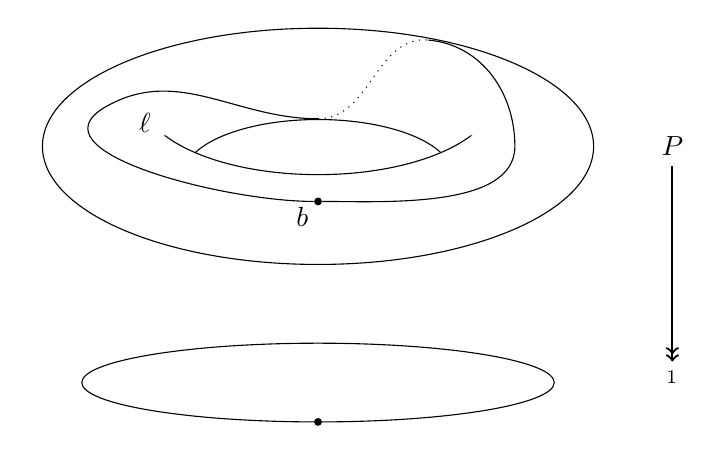
\begin{tikzpicture}
    \draw (0,0) ellipse (3 and .5);
    \draw (0,3) ellipse (3.5 and 1.5);
    \begin{scope}[yshift=4]
      \clip (-3,3) -- (-1.8,3) -- (-1.8,3.7) -- (1.8,3.7) -- (1.8,3) -- (3,3) -- (3,0) -- (-3,0) -- cycle;
      \draw[clip] (0,3.5) ellipse (2.25 and 1);
      \draw (0,2.5) ellipse (1.7 and .7);
    \end{scope}
    \node (P) at (4.5,3) {$P$};
    \node (S1) at (4.5,0) {$\Sn^1$};
    \draw[->>,thick] (P) -- (S1);
    \node[fill,circle,inner sep=1pt,label={below right:$\base$}] at (0,-.5) {};
    \node at (-2.6,.6) {$\lloop$};
    \node[fill,circle,\OPTblue,inner sep=1pt] (b) at (0,2.3) {};
    \node[\OPTblue] at (-.2,2.1) {$b$};
    \begin{scope}
      \draw[\OPTblue] (b) to[out=180,in=-150] (-2.7,3.5) to[out=30,in=180] (0,3.35);
      \draw[\OPTblue,dotted] (0,3.35) to[out=0,in=175] (1.4,4.35);
      \draw[\OPTblue] (1.4,4.35) to[out=-5,in=90] (2.5,3) to[out=-90,in=0,looseness=.8] (b);
    \end{scope}
    \node[\OPTblue] at (-2.2, 3.3) {$\ell$};
  \end{tikzpicture}
  \caption{圆周 $\Sn^1$ 的拓扑归纳原则}
  \label{fig:topS1ind}
\end{figure}

\begin{figure}
  \centering
  \begin{tikzpicture}
    \draw (0,0) ellipse (3 and .5);
    \draw (0,3) ellipse (3.5 and 1.5);
    \begin{scope}[yshift=4]
      \clip (-3,3) -- (-1.8,3) -- (-1.8,3.7) -- (1.8,3.7) -- (1.8,3) -- (3,3) -- (3,0) -- (-3,0) -- cycle;
      \draw[clip] (0,3.5) ellipse (2.25 and 1);
      \draw (0,2.5) ellipse (1.7 and .7);
    \end{scope}
    \node (P) at (4.5,3) {$P$};
    \node (S1) at (4.5,0) {$\Sn^1$};
    \draw[->>,thick] (P) -- (S1);
    \node[fill,circle,inner sep=1pt,label={below right:$\base$}] at (0,-.5) {};
    \node at (-2.6,.6) {$\lloop$};
    \node[fill,circle,\OPTblue,inner sep=1pt] (b) at (0,2.3) {};
    \node[\OPTblue] at (-.3,2.3) {$b$};
    \node[fill,circle,\OPTpurple,inner sep=1pt] (tb) at (0,1.8) {};
    % \draw[\OPTpurple,dashed] (b) to[out=0,in=0,looseness=5] (0,4) to[out=180,in=180] (tb);
    \draw[\OPTpurple,dashed] (b) arc (-90:90:2.9 and 0.85) arc (90:270:2.8 and 1.1);
    \begin{scope}
      \clip (b) -- ++(.1,0) -- (.1,1.8) -- ++(-.2,0) -- ++(0,-1) -- ++(3,2) -- ++(-3,0) -- (-.1,2.3) -- cycle;
      \draw[\OPTred,dotted,thick] (.2,2.07) ellipse (.2 and .57);
      \begin{scope}
        % \draw[clip] (b) -- ++(.1,0) |- (tb) -- ++(-.2,0) -- ++(0,-1) -| ++(3,3) -| (b);
        \clip (.2,0) rectangle (-2,3);
        \draw[\OPTred,thick] (.2,2.07) ellipse (.2 and .57);
      \end{scope}
    \end{scope}
    \node[\OPTred] at (1,1.2) {$\ell: \trans \lloop b=b$};
  \end{tikzpicture}
  \caption{圆周 $\Sn^1$ 的类型论归纳原则}
  \label{fig:ttS1ind}
\end{figure}

当然,我们期望可以通过将 $P$ 设为常类型族来从归纳原则推导出递归原则。事实上确实如此,尽管从依赖的 $\lloop$ 计算规则(它涉及 $\apdfunc f$)推导出非依赖的计算规则(它涉及 $\apfunc f$)出人意料地有点棘手。

\begin{lem}\label{thm:S1rec}
\index{递归原则!for S1@for $\Sn^1$}%
\index{计算规则!for S1@for $\Sn^1$}%
如果 $A$ 是一个带有 $a:A$ 和 $p:\id[A]aa$ 的类型,那么存在一个
函数 $f:\Sn^1\to{}A$ 使得
\begin{align*}
  f(\base)&\defeq a \\
  \apfunc f(\lloop)&\defid p.
\end{align*}
\end{lem}
\begin{proof}
  我们想要将 $\Sn^1$ 的归纳原则应用于常类型族 $(\lam{x} A): \Sn^1\to \UU$。为此所需的假设是 $(\lam{x} A)(\base) \jdeq A$ 的一点,我们有(即 $a:A$),以及 $\dpath {x \mapsto A}{\lloop} a a$ 中的一个依赖路径,或等价地 $\transfib{x \mapsto A}{\lloop} a = a$。该类型与 $p$ 所在的类型 $\id[A]aa$ 不同,但它等价于后者,因为根据 \cref{thm:trans-trivial} 我们有 $\transconst{A}{\lloop}{a} : \transfib{x \mapsto A}{\lloop} a= a$。因此,给定 $a:A$ 和 $p:a=a$,我们可以考虑复合
  \[\transconst{A}{\lloop}{a} \ct p:(\dpath {x \mapsto A}\lloop aa)。\]
  应用归纳原则,我们得到 $f:\Sn^1\to A$ 使得
  \begin{align}
    f(\base) &\jdeq a \qquad\text{and}\label{eq:S1recindbase}\\
    \apdfunc f(\lloop) &= \transconst{A}{\lloop}{a} \ct p。\label{eq:S1recindloop}
  \end{align}
  现在需要推导出 $\apfunc f(\lloop)=p$ 等式。然而,根据 \cref{thm:apd-const},我们有
  \[\apdfunc f(\lloop) = \transconst{A}{\lloop}{f(\base)} \ct \apfunc f(\lloop)。\]
  将此与~\eqref{eq:S1recindloop} 结合,并取消 $\transconstf$ 的出现(根据~\eqref{eq:S1recindbase} 它们是相同的),我们得到 $\apfunc f(\lloop)=p$。
\end{proof}

% 同样,在这种情况下,我们将通过 $f(\base)\defeq a$ 和 $\ap f \lloop \defid p$ 定义的 $f$ 视为定义。
我们还有一个相应的唯一性原则。

\begin{lem}\label{thm:uniqueness-for-functions-on-S1}
\index{唯一性!原则,命题性!对于圆周上的函数}%
如果 $A$ 是一个类型,且 $f,g:\Sn^1\to{}A$ 是两个映射,$p,q$ 是两个
等式:
\begin{align*}
  p:f(\base)&=_Ag(\base),\\
  q:\map{f}\lloop&=^{\lam{x} x=_Ax}_p\map{g}\lloop。
\end{align*}
那么对于所有 $x:\Sn^1$,我们有 $f(x)=g(x)$。
\end{lem}
\begin{proof}
  我们在类型族 $P(x)\defeq(f(x)=g(x))$ 处应用 $\Sn^1$ 的归纳原则。当 $x$ 为 $\base$ 时,$p$ 正是我们需要的。当 $x$ 沿 $\lloop$ 变化时,我们需要
  \(p=^{\lam{x} f(x)=g(x)}_{\lloop} p,\)
  根据 \cref{thm:transport-path,thm:dpath-path} 这一点可以简化为 $q$。
\end{proof}

\index{universal!property!of S1@of $\Sn^1$}%
这两个引理暗示了圆周的预期普遍性质:

\begin{lem}\label{thm:S1ump}
对于任何类型 $A$,我们有一个自然的等价
\[ (\Sn^1 \to A) \;\eqvsym\;
\sm{x:A} (x=x)。
\]
\end{lem}
\begin{proof}
  我们有一个标准函数 $f:(\Sn^1 \to A) \to \sm{x:A} (x=x)$,定义为 $f(g) \defeq (g(\base),\ap g \lloop)$。反过来,我们有 $g:\sm{x:A} (x=x) \to (\Sn^1 \to A)$,定义为将一对 $(b,\ell)$ 变为由圆周的递归原则给出的函数 $\Sn^1 \to A$。

  现在,通过圆周递归原则的计算规则,$f \circ g \htpy \idfunc$。而且通过唯一性原则,由于\((g \circ f)(\lloop) =^{\lam{x} x=_Ax}_{\refl{\base}} \lloop\),再加上圆周递归原则的计算规则,$g \circ f \htpy \idfunc$。因此,$f$ 有一个准逆元 (quasi-inverse),因此是一个等价。
\end{proof}

\index{type!circle|)}%

与 \cref{sec:htpy-inductive} 中一样,我们可以表明 \cref{thm:S1ump} 的结论等价于具有命题性计算规则的归纳原则。其他高阶归纳类型也满足类似于 \cref{thm:S1rec,thm:S1ump} 的引理;我们通常会将它们的证明留给读者。现在我们继续考虑许多示例。

\section{区间 (The interval)}
\label{sec:interval}

\index{类型!区间|(defstyle}%
\indexsee{区间!类型}{type, interval}%
\define{区间 (interval)},我们记作 $\interval$,它可能比圆更简单的高阶归纳类型。
它由以下部分生成:
\begin{itemize}
  \item 一个点 $\izero:\interval$,
  \item 一个点 $\ione:\interval$, 和
  \item 一条路径 $\seg : \id[\interval]\izero\ione$.
\end{itemize}
\index{递归原理!区间类型}%
区间的递归原理表明,给定一个类型 $B$ 以及
\begin{itemize}
  \item 一个点 $b_0:B$,
  \item 一个点 $b_1:B$, 和
  \item 一条路径 $s:b_0=b_1$,
\end{itemize}
存在一个函数 $f:\interval\to B$ 使得 $f(\izero)\jdeq b_0$, $f(\ione)\jdeq b_1$, 并且 $\ap f \seg = s$。
\index{归纳原理!区间类型}%
归纳原理表明,给定 $P:\interval\to\type$ 以及
\begin{itemize}
  \item 一个点 $b_0:P(\izero)$,
  \item 一个点 $b_1:P(\ione)$, 和
  \item 一条路径 $s:\dpath{P}{\seg}{b_0}{b_1}$,
\end{itemize}
存在一个函数 $f:\prd{x:\interval} P(x)$ 使得 $f(\izero)\jdeq b_0$, $f(\ione)\jdeq b_1$, 并且 $\apd f \seg = s$。

纯粹从同伦角度来看,区间并不是真的有趣:

\begin{lem}\label{thm:contr-interval}
类型 $\interval$ 是可约的。
\end{lem}

\begin{proof}
  我们证明对所有 $x:\interval$,我们有 $x=_\interval\ione$。换句话说,我们希望有一个
  函数 $f$ 的类型为 $\prd{x:\interval}(x=_\interval\ione)$。我们开始定义 $f$,如下所示:
  \begin{alignat*}{2}
    f(\izero)&\defeq \seg  &:\izero&=_\interval\ione,\\
    f(\ione)&\defeq \refl\ione &:\ione &=_\interval\ione.
  \end{alignat*}
  剩下的就是定义 $\apd{f}\seg$,它必须具有类型 $\seg =_\seg^{\lam{x} x=_\interval\ione}\refl \ione$。
  根据定义,这个类型是 $\trans\seg\seg=_{\ione=_\interval\ione}\refl\ione$,其结果等价于 $\rev\seg\ct\seg=\refl\ione$。
  但该类型中有一个规范元素,即路径逆元实际上是逆元的证明。
\end{proof}

然而,从类型论的角度来看,区间仍然具有一些有趣的特性,类似于经典同伦论中的拓扑区间。
例如,它使我们能够给出函数外延性(function extensionality)的简单证明。
(当然,正如 \cref{sec:univalence-implies-funext} 所述,在下面的证明期间,我们暂停使用函数外延性公理的整体假设。)

\begin{lem}\label{thm:interval-funext}
\index{函数外延性!由区间类型证明}%
如果 $f,g:A\to{}B$ 是两个函数,并且对每个 $x:A$,$f(x)=g(x)$,那么
$f=g$ 在类型 $A\to{}B$ 中成立。
\end{lem}

\begin{proof}
  我们称已有的证明为 $p:\prd{x:A}(f(x)=g(x))$。对于所有 $x:A$,我们定义
  一个函数 $\widetilde{p}_x:\interval\to{}B$ 如下:
  \begin{align*}
    \widetilde{p}_x(\izero) &\defeq f(x), \\
    \widetilde{p}_x(\ione) &\defeq g(x), \\
    \map{\widetilde{p}_x}\seg &\defid p(x).
  \end{align*}
  我们现在定义 $q:\interval\to(A\to{}B)$ 如下:
  \[q(i)\defeq(\lam{x} \widetilde{p}_x(i))\]
  那么 $q(\izero)$ 是函数 $\lam{x} \widetilde{p}_x(\izero)$,它等于 $f$,因为 $\widetilde{p}_x(\izero)$ 是由 $f(x)$ 定义的。
  同样地,我们有 $q(\ione)=g$,因此
  \[\map{q}\seg:f=_{(A\to{}B)}g \qedhere\]
\end{proof}

在 \cref{ex:funext-from-interval} 中,我们要求读者从 \cref{thm:interval-funext} 完成函数外延性公理的完整证明。

\index{类型!区间|)}%

\section{圆和球 (Circles and spheres)}
\label{sec:circle}

\index{类型!圆|(}%
我们已经讨论过圆 $\Sn^1$ 作为高阶归纳类型,它由以下部分生成:
\begin{itemize}
  \item 一个点 $\base:\Sn^1$, 和
  \item 一条路径 $\lloop : {\id[\Sn^1]\base\base}$.
\end{itemize}
\index{归纳原理!S1@对 $\Sn^1$ 的归纳原理}%
它的归纳原理表明,给定 $P:\Sn^1\to\type$,以及 $b:P(\base)$ 和 $\ell :\dpath P \lloop b b$,我们有 $f:\prd{x:\Sn^1} P(x)$,并且 $f(\base)\jdeq b$ 且 $\apd f \lloop = \ell$。
它的非依赖递归原理表明,给定 $B$ 以及 $b:B$ 和 $\ell:b=b$,我们有 $f:\Sn^1\to B$,并且 $f(\base)\jdeq b$ 且 $\ap f \lloop = \ell$。

我们观察到圆是非平凡的。

\begin{lem}\label{thm:loop-nontrivial}
$\lloop\neq\refl{\base}$。
\end{lem}
\begin{proof}
  假设 $\lloop=\refl{\base}$。
  然后,由于对于任何带有 $x:A$ 和 $p:x=x$ 的类型 $A$,存在一个函数 $f:\Sn^1\to A$ 定义为 $f(\base)\defeq x$ 且 $\ap f \lloop \defid p$,我们有
  \[p = f(\lloop) = f(\refl{\base}) = \refl{x}。\]
  但这意味着每种类型都是一个集合,正如我们所见,这并不成立(见 \cref{thm:type-is-not-a-set})。
\end{proof}

圆还具有以下有趣的特性,它作为反例的来源非常有用。

\begin{lem}\label{thm:S1-autohtpy}
存在一个元素 $\prd{x:\Sn^1} (x=x)$,它不等于 $x\mapsto \refl{x}$。
\end{lem}
\begin{proof}
  我们通过 $\Sn^1$-归纳定义 $f:\prd{x:\Sn^1} (x=x)$。
  当 $x$ 是 $\base$ 时,我们设 $f(\base)\defeq \lloop$。
  现在,当 $x$ 沿着 $\lloop$ 变化时(见 \cref{rmk:varies-along}),我们必须证明 $\transfib{x\mapsto x=x}{\lloop}{\lloop} = \lloop$。
  然而,在 \cref{sec:compute-paths} 中,我们观察到 $\transfib{x\mapsto x=x}{p}{q} = \opp{p} \ct q \ct p$,所以我们需要证明的是 $\opp{\lloop} \ct \lloop \ct \lloop = \lloop$。
  但是,通过消去逆元,这显然是正确的。

  要证明 $f\neq (x\mapsto \refl{x})$,我们只需证明 $f(\base) \neq \refl{\base}$。
  但 $f(\base)=\lloop$,所以这正是前一个引理的内容。
\end{proof}

例如,这使我们能够扩展 \cref{thm:type-is-not-a-set},表明包含圆的任何宇宙都不能是一个1-型(1-type)。

\begin{cor}
  如果类型 $\Sn^1$ 属于某个宇宙 \type,那么 \type 不是一个1-型。
\end{cor}
\begin{proof}
  类型 $\Sn^1=\Sn^1$ 在 \type 中,通过一值性,可以等价于 $\Sn^1$ 的自等价类型 $\eqv{\Sn^1}{\Sn^1}$,所以只需证明 $\eqv{\Sn^1}{\Sn^1}$ 不是一个集合。
  \index{自同构!S1@对 $\Sn^1$ 的自同构}%
  为此,只需证明其等式类型 $\id[(\eqv{\Sn^1}{\Sn^1})]{\idfunc[\Sn^1]}{\idfunc[\Sn^1]}$ 不是一个单纯命题(mere proposition)。
  由于作为等价是一个单纯命题,这个类型等价于 $\id[(\Sn^1\to\Sn^1)]{\idfunc[\Sn^1]}{\idfunc[\Sn^1]}$。
  但通过函数外延性,这等价于 $\prd{x:\Sn^1} (x=x)$,正如我们在 \cref{thm:S1-autohtpy} 中所见,其中包含两个不相等的元素。
\end{proof}

\index{类型!圆|)}%

\index{类型!2-球|(}%
\indexsee{球类型}{type, sphere}%
我们还提到,2-球 $\Sn^2$ 应该是高阶归纳类型,由以下部分生成:
\symlabel{s2b}
\begin{itemize}
  \item 一个点 $\base:\Sn^2$, 和
  \item 一个 2 维路径 $\surf:\refl{\base} = \refl{\base}$ 在 ${\base=\base}$ 中。
\end{itemize}
\index{递归原理!S2@对 $\Sn^2$ 的递归原理}%
对于 $\Sn^2$ 的递归原理并不难:它表明给定 $B$,其中 $b:B$ 和 $s:\refl b = \refl b$,我们有 $f:\Sn^2\to B$,其中 $f(\base)\jdeq b$ 且 $\aptwo f \surf = s$。
这里 ``$\aptwo f \surf$'' 表示将 $f$ 的函子性扩展到二维路径的操作,可以精确地表述如下。

\begin{lem}\label{thm:ap2}
给定 $f:A\to B$ 和 $x,y:A$ 以及 $p,q:x=y$ 和 $r:p=q$,我们有路径 $\aptwo f r : \ap f p = \ap f q$。
\end{lem}
\begin{proof}
  通过路径归纳法,我们可以假设 $p\jdeq q$ 并且 $r$ 是反射性。
  但此时我们可以定义 $\aptwo f {\refl p} \defeq \refl{\ap f p}$。
\end{proof}

为了陈述一般的归纳原理,我们需要该引理的依赖函数版本,这反过来需要依赖二维路径的概念。
如前所述,有多种方式来定义这种事物;其中一种方式是通过传输的二维版本。

\begin{lem}\label{thm:transport2}
给定 $P:A\to\type$ 和 $x,y:A$ 以及 $p,q:x=y$ 和 $r:p=q$,对于任何 $u:P(x)$,我们有 $\transtwo r u : \trans p u = \trans q u$。
\end{lem}
\begin{proof}
  通过路径归纳法。
\end{proof}

现在,假设给定 $x,y:A$ 和 $p,q:x=y$ 以及 $r:p=q$,还有点 $u:P(x)$ 和 $v:P(y)$,以及依赖路径 $h:\dpath P p u v$ 和 $k:\dpath P q u v$。
根据我们对依赖路径的定义,这意味着 $h:\trans p u = v$ 和 $k:\trans q u = v$。
因此,将依赖二维路径的类型定义为
\[ (\dpath P r h k )\defeq (h = \transtwo r u \ct k)。\]
我们现在可以陈述 \cref{thm:ap2} 的依赖版本。

\begin{lem}\label{thm:apd2}
给定 $P:A\to\type$ 和 $x,y:A$ 以及 $p,q:x=y$ 和 $r:p=q$ 以及一个函数 $f:\prd{x:A} P(x)$,我们有
$\apdtwo f r : \dpath P r {\apd f p}{\apd f q}$。
\end{lem}
\begin{proof}
  路径归纳。
\end{proof}

\index{归纳原理!S2@对 $\Sn^2$ 的归纳原理}%
现在我们可以陈述 $\Sn^2$ 的归纳原理:假设给定 $P:\Sn^2\to\type$,其中 $b:P(\base)$ 和 $s:\dpath Q \surf {\refl b}{\refl b}$,其中 $Q\defeq\lam{p} \dpath P p b b$。然后存在一个函数 $f:\prd{x:\Sn^2} P(x)$ 使得 $f(\base)\jdeq b$ 并且 $\apdtwo f \surf = s$。

\index{类型!2-球|)}%

当然,这种显式的方法随着维度的升高变得越来越复杂。
因此,如果我们想为所有 $n$ 定义 $n$-球,我们需要一些更系统的方法。
一种方法是直接处理 $n$-维循环($n$-dimensional loops)\index{循环!n-@$n$-},而不是一般的 $n$-维路径。\index{路径!n-@$n$-}

\index{类型!点化类型}%
回顾 \cref{sec:equality} 中 \emph{点化类型 (pointed types)} $\type_*$ 的定义,以及 $n$ 次循环空间\index{循环空间!迭代} $\Omega^n : \type_* \to \type_*$
(\cref{def:pointedtype,def:loopspace})。现在我们可以定义
$n$-球 $\Sn^n$ 作为由以下部分生成的高阶归纳类型
\index{类型!n-球@$n$-球}%
\begin{itemize}
  \item 一个点 $\base:\Sn^n$, 和
  \item 一个 $n$-循环 $\lloop_n : \Omega^n(\Sn^n,\base)$。
\end{itemize}
为了写出这种表示的归纳原理,我们需要定义 ``依赖 $n$-循环 (dependent $n$-loop)\indexdef{循环!依赖的 n-@依赖的 $n$-}'' 的概念,以及依赖函数对 $n$-循环的作用。
我们将此留给读者(见 \cref{ex:nspheres});在下一节中,我们将讨论一种不同的定义球的方法,有时更易于处理。

\section{悬挂 (Suspensions)}
\label{sec:suspension}

\indexsee{类型!悬挂}{suspension}%
\index{悬挂|(defstyle}%
类型 $A$ 的 \define{悬挂 (suspension)} 是使 $A$ 的点变为路径的通用方式(因此 $A$ 中的路径变为 2-路径,以此类推)。
它是一个类型 $\susp A$,由以下生成器定义:\footnote{这里有一个不幸的符号冲突,依赖对类型对也用 $\Sigma$ 表示。
然而,通常上下文可以消除歧义。}
\begin{itemize}
  \item 一个点 $\north:\susp A$,
  \item 一个点 $\south:\susp A$, 和
  \item 一个函数 $\merid:A \to (\id[\susp A]\north\south)$。
\end{itemize}
这些名称意在表明某种 ``球体'',具有北极、南极,以及从一个极点到另一个极点的一组 $A$ 的子午线
\indexdef{极点}%
\indexdef{子午线}%
。实际上,正如我们将看到的,如果 $A=\Sn^1$,那么它的悬挂等价于普通球面的表面,即 $\Sn^2$。

\index{递归原理!悬挂}%
悬挂的递归原理表明,给定类型 $B$ 以及
\begin{itemize}
  \item 点 $n,s:B$ 和
  \item 函数 $m:A \to (n=s)$,
\end{itemize}
我们有一个函数 $f:\susp A \to B$ 使得 $f(\north)\jdeq n$ 和 $f(\south)\jdeq s$,并且对所有 $a:A$,我们有 $\ap f {\merid(a)} = m(a)$。
\index{归纳原理!悬挂}%
类似地,归纳原理表明,给定 $P:\susp A \to \type$,并且
\begin{itemize}
  \item 一个点 $n:P(\north)$,
  \item 一个点 $s:P(\south)$, 和
  \item 对每个 $a:A$,一条路径 $m(a):\dpath P{\merid(a)}ns$,
\end{itemize}
存在一个函数 $f:\prd{x:\susp A} P(x)$ 使得 $f(\north)\jdeq n$,$f(\south)\jdeq s$,并且对每个 $a:A$,我们有 $\apd f {\merid(a)} = m(a)$。

我们的第一个关于悬挂的观察是,它提供了另一种定义圆的方法。

\begin{lem}\label{thm:suspbool}
\index{类型!圆}%
$\eqv{\susp\bool}{\Sn^1}$。
\end{lem}
\begin{proof}
  定义 $f:\susp\bool\to\Sn^1$ 通过递归使得 $f(\north)\defeq \base$ 和 $f(\south)\defeq\base$,同时 $\ap f{\merid(\bfalse)}\defid\lloop$,但 $\ap f{\merid(\btrue)} \defid \refl{\base}$。
  定义 $g:\Sn^1\to\susp\bool$ 通过递归使得 $g(\base)\defeq \north$ 并且 $\ap g \lloop \defid \merid(\bfalse) \ct \opp{\merid(\btrue)}$。
  我们现在展示 $f$ 和 $g$ 是准逆元。

  首先,我们通过归纳证明 $g(f(x))=x$ 对所有 $x:\susp \bool$ 成立。
  如果 $x\jdeq\north$,那么 $g(f(\north)) \jdeq g(\base)\jdeq \north$,所以我们有 $\refl{\north} : g(f(\north))=\north$。
  如果 $x\jdeq\south$,那么 $g(f(\south)) \jdeq g(\base)\jdeq \north$,并且我们选择等式 $\merid(\btrue) : g(f(\south)) = \south$。
  剩下的就是展示,对于任何 $y:\bool$,当 $x$ 沿着 $\merid(y)$ 变化时,这些等式是保持的,这就是说,当 $\refl{\north}$ 沿着 $\merid(y)$ 传输时,它产生 $\merid(\btrue)$。
  通过路径空间和拉回纤维丛中的传输,这意味着我们需要证明
  \[ \opp{\ap g {\ap f {\merid(y)}}} \ct \refl{\north} \ct \merid(y) = \merid(\btrue)。\]
  当然,我们可以消除 $\refl{\north}$。
  现在通过 \bool-归纳法,我们可以假设 $y\jdeq \bfalse$ 或者 $y\jdeq \btrue$。
  如果 $y\jdeq \bfalse$,那么我们有
  \begin{align*}
    \opp{\ap g {\ap f {\merid(\bfalse)}}} \ct \merid(\bfalse)
    &= \opp{\ap g {\lloop}} \ct \merid(\bfalse)\\
    &= \opp{(\merid(\bfalse) \ct \opp{\merid(\btrue)})} \ct \merid(\bfalse)\\
    &= \merid(\btrue) \ct \opp{\merid(\bfalse)} \ct \merid(\bfalse)\\
    &= \merid(\btrue)
  \end{align*}
  而如果 $y\jdeq \btrue$,那么我们有
  \begin{align*}
    \opp{\ap g {\ap f {\merid(\btrue)}}} \ct \merid(\btrue)
    &= \opp{\ap g {\refl{\base}}} \ct \merid(\btrue)\\
    &= \opp{\refl{\north}} \ct \merid(\btrue)\\
    &= \merid(\btrue)。
  \end{align*}
  因此,对于所有 $x:\susp \bool$,我们有 $g(f(x))=x$。

  现在我们通过归纳证明 $f(g(x))=x$ 对所有 $x:\Sn^1$ 成立。
  如果 $x\jdeq \base$,那么 $f(g(\base))\jdeq f(\north)\jdeq\base$,所以我们有 $\refl{\base} : f(g(\base))=\base$。
  剩下的就是展示,当 $x$ 沿着 $\lloop$ 变化时,这个等式是保持的,这就是说,它沿着 $\lloop$ 传输到它自身。
  同样地,通过路径空间和拉回纤维丛中的传输,这意味着需要证明
  \[ \opp{\ap f {\ap g {\lloop}}} \ct \refl{\base} \ct \lloop = \refl{\base}。\]
  然而,我们有
  \begin{align*}
    \ap f {\ap g {\lloop}} &= \ap f {\merid(\bfalse) \ct \opp{\merid(\btrue)}}\\
    &= \ap f {\merid(\bfalse)} \ct \opp{\ap f {\merid(\btrue)}}\\
    &= \lloop \ct \refl{\base}
  \end{align*}
  因此这很容易跟随。
\end{proof}

从拓扑学上讲,二点空间 \bool 也被称为 \emph{0 维球 (0-dimensional sphere)},$\Sn^0$。
(例如,它是 $\mathbb{R}^1$ 中距离原点为 1 的点集,正如拓扑 1-球是 $\mathbb{R}^2$ 中距离原点为 1 的点集一样。)
因此,\cref{thm:suspbool} 可以暗示性地表述为 $\eqv{\susp\Sn^0}{\Sn^1}$。
\index{类型!n-球@$n$-球|defstyle}%
\indexsee{n-球@$n$-球}{type, $n$-sphere}%
实际上,这个模式继续:我们可以通过递归定义所有的球
\begin{equation}\label{eq:Snsusp}
\Sn^0 \defeq \bool
\qquad\text{并且}\qquad
\Sn^{n+1} \defeq \susp \Sn^n。
\end{equation}
我们甚至可以从低一维开始定义 $\Sn^{-1}\defeq \emptyt$,并观察到 $\eqv{\susp\emptyt}{\bool}$。

要仔细证明这与上一节中的 $\Sn^n$ 的定义一致,需要使后者更加明确。
然而,我们可以证明递归定义具有我们期望另一种定义应具有的相同的通用性质。
如果 $(A,a_0)$ 和 $(B,b_0)$ 是点化类型(基点通常隐式地保留),则令 $\Map_*(A,B)$ 表示基映射类型:
\index{基映射}
\symlabel{基映射}
\[ \Map_*(A,B) \defeq \sm{f:A\to B} (f(a_0)=b_0)。\]
注意,任何类型 $A$ 都可以产生一个点化类型 $A_+ \defeq A+\unit$,基点为 $\inr(\ttt)$;这称为 \emph{添加一个不相交的基点}。
\indexdef{基点!添加一个不相交的}%
\index{不相交!基点}%
\index{添加一个不相交的基点}%

\begin{lem}
  对于类型 $A$ 和点化类型 $(B,b_0)$,我们有
  \[ \eqv{\Map_*(A_+,B)}{(A\to B)}。\]
\end{lem}
注意,在右边我们有普通的 \emph{非点化} 函数的类型从 $A$ 到 $B$。
\begin{proof}
  从左到右,给定 $f:A_+ \to B$,其中 $p:f(\inr(\ttt)) = b_0$,我们有 $f\circ \inl : A \to B$。
  从右到左,给定 $g:A\to B$,我们定义 $g':A_+ \to B$ 通过 $g'(\inl(a))\defeq g(a)$ 和 $g'(\inr(u)) \defeq b_0$。
  我们留给读者证明这些是准逆操作。
\end{proof}

特别地,注意到 $\eqv{\bool}{\unit_+}$。
因此,对于任何点化类型 $B$,我们有
\[{\Map_*(\bool,B)} \eqvsym {(\unit \to B)}\eqvsym B。\]
%
现在回顾循环空间\index{循环空间}操作 $\Omega$ 作用于点化类型,定义 $\Omega(A,a_0) \defeq (\id[A]{a_0}{a_0},\refl{a_0})$。
我们也可以使悬挂 $\susp$ 作用于点化类型,通过 $\susp(A,a_0)\defeq (\susp A,\north)$。

\begin{lem}\label{lem:susp-loop-adj}
\index{悬挂的通用性质}%
对于点化类型 $(A,a_0)$ 和 $(B,b_0)$ 我们有
\[ \eqv{\Map_*(\susp A, B)}{\Map_*(A,\Omega B)}。\]
\end{lem}
\addtocounter{thm}{1}           % 因为我们在 commit 8f54d16 中移除了编号方程
\begin{proof}
  我们首先观察到以下一系列等价关系:
  \begin{align*}
    \Map_*(\susp A, B) & \defeq \sm{f:\susp A\to B} (f(\north)=b_0) \\
    & \eqvsym \sm{f:\sm{b_n : B}{b_s : B} (A \to (b_n = b_s))} (\fst(f)=b_0) \\
    & \eqvsym \sm{b_n : B}{b_s : B} \big(A \to (b_n = b_s)\big) \times (b_n=b_0) \\
    & \eqvsym \sm{p : \sm{b_n : B} (b_n=b_0)}{b_s : B} (A \to (\fst(p) = b_s)) \\
    & \eqvsym \sm{b_s : B} (A \to (b_0 = b_s))
  \end{align*}
  第一个等价关系是通过悬挂的通用性质,它表明
  \[ \Parens{\susp A \to B} \eqvsym \Parens{\sm{b_n : B} \sm{b_s : B} (A \to (b_n = b_s)) } \]
  从右到左的函数由递归器给出(见 \cref{ex:susp-lump})。
  第二个和第三个等价关系是通过 \cref{ex:sigma-assoc},以及组件的重新排序。
  最后一个等价关系是通过 \cref{thm:omit-contr},因为根据 \cref{thm:contr-paths},$\sm{b_n : B} (b_n=b_0)$ 是可约的,中心为 $(b_0, \refl{b_0})$。

  现在通过以下等价链完成证明:
  \begin{align*}
    \sm{b_s : B} (A \to (b_0 = b_s))
    &\eqvsym \sm{b_s : B}{g:A \to (b_0 = b_s)}{q:b_0 = b_s} (g(a_0) = q)\\
    &\eqvsym \sm{r : \sm{b_s : B}(b_0 = b_s)}{g:A \to (b_0 = \proj1(r))} (g(a_0) = \proj2(r))\\
    &\eqvsym \sm{g:A \to (b_0 = b_0)} (g(a_0) = \refl{b_0})\\
    &\jdeq \Map_*(A,\Omega B)。
  \end{align*}
  类似于之前,第一个和最后一个等价关系通过 \cref{thm:omit-contr,thm:contr-paths},第二个通过 \cref{ex:sigma-assoc} 和组件的重新排序。
\end{proof}

\index{类型!n-球@$n$-球|defstyle}%
特别地,对于按 \eqref{eq:Snsusp} 定义的球,我们有
\index{Sn@of $\Sn^n$ 的通用性质}%
\[ \Map_*(\Sn^n,B) \eqvsym \Map_*(\Sn^{n-1}, \Omega B) \eqvsym \cdots \eqvsym \Map_*(\bool,\Omega^n B) \eqvsym \Omega^n B。\]
因此,这些 $\Sn^n$ 具有我们期望从 \cref{sec:circle} 中直接基于 $n$ 次循环空间\index{循环空间!迭代} 定义的球应具有的通用性质。

\index{悬挂|)}%
\section{胞腔复形 (Cell complexes)}
\label{sec:cell-complexes}

\index{胞腔复形|(defstyle}%
\index{CW 复形|(defstyle}%
在经典拓扑学中,\emph{胞腔复形 (cell complex)} 是通过逐步将圆盘沿其边界附加而得到的空间。
如果一个 $n$ 维圆盘的边界\index{圆盘}被限制在严格低于 $n$ 维的圆盘内(即 $(n-1)$ 骨架 (skeleton)),则该空间称为 \emph{CW 复形 (CW complex)}。\index{CW 骨架!CW 复形的骨架}

任何有限 CW 复形都可以表示为一个高阶归纳类型 (higher inductive type),通过将 $n$ 维圆盘转化为 $n$ 维路径,并将附加映射 (attaching map)\index{附加映射}的像分为路径构造器 (path constructor) 的源 (source)\index{源!路径构造器的源}和目标 (target)\index{目标!路径构造器的目标},每个都写成低维路径的组合。
我们在 \cref{sec:circle} 中对 $\Sn^1$ 和 $\Sn^2$ 的明确定义具有这种形式。

\index{圆环}%
另一个例子是圆环 $T^2$,它由以下生成:
\begin{itemize}
  \item 一个点 $b:T^2$,
  \item 一条路径 $p:b=b$,
  \item 另一条路径 $q:b=b$, 以及
  \item 一个 2-路径 $t: p\ct q = q \ct p$。
\end{itemize}
也许看出这是一个圆环的最简单方法是从一个矩形开始,它有四个角 $a,b,c,d$,四条边 $p,q,r,s$,以及一个内部路径,它显然是从 $p\ct q$ 到 $r\ct s$ 的 2-路径 $t$:
\begin{equation*}
  \xymatrix{
    a\ar@{=}[r]^p\ar@{=}[d]_r \ar@{}[dr]|{\Downarrow t} &
    b\ar@{=}[d]^q\\
    c\ar@{=}[r]_s &
    d
  }
\end{equation*}
现在将边 $r$ 与 $q$ 以及边 $s$ 与 $p$ 识别,从而也识别了所有四个角。
在拓扑学上,可以看出这种识别产生了一个圆环。

\index{归纳原理!圆环}%
\index{圆环!圆环的归纳原理}%
对于圆环的归纳原理是我们到目前为止写出的最棘手的一个。
给定 $P:T^2\to\type$,对于截面 $\prd{x:T^2} P(x)$,我们需要
\begin{itemize}
  \item 一个点 $b':P(b)$,
  \item 一条路径 $p' : \dpath P p {b'} {b'}$,
  \item 一条路径 $q' : \dpath P q {b'} {b'}$, 以及
  \item 一个 2-路径 $t'$,在 $t$ 上方连接复合路径 $p'\ct q'$ 和 $q'\ct p'$。
\end{itemize}
为了理解这最后的数据,我们需要一个依赖路径的复合操作,但这并不难定义。
然后,归纳原理给出一个函数 $f:\prd{x:T^2} P(x)$ 使得 $f(b)\jdeq b'$ 且 $\apd f {p} = p'$ 和 $\apd f {q} = q'$ 并且类似于 ``$\apdtwo f t = t'$'' 的等式。
然而,这在目前状态下是类型不正确的,首先是因为等式 $\apd f {p} = p'$ 和 $\apd f {q} = q'$ 不是判断等式 (judgmental equality),其次是因为 $\apdfunc f$ 仅在同伦 (homotopy) 意义上保留路径的连接。
我们将细节留给读者(见 \cref{ex:torus})。

当然,圆环的另一个定义是 $T^2 \defeq \Sn^1 \times \Sn^1$(在 \cref{ex:torus-s1-times-s1} 中,我们要求读者验证这两个定义的等价性)。
\index{克莱因瓶}%
\index{射影平面}%
然而,胞腔复形的定义很容易推广到其他没有这样描述的空间,例如克莱因瓶 (Klein bottle)、射影平面 (projective plane) 等等。
但是,书写归纳原理变得越来越困难,要求我们定义依赖 $n$-路径和 $\apdfunc{}$ 作用于 $n$-路径的概念。
幸运的是,一旦我们掌握了球面 (spheres),就有办法绕过这个问题。

\section{中心与辐条 (Hubs and spokes)}
\label{sec:hubs-spokes}

\indexsee{辐条}{中心与辐条}%
\index{中心与辐条|(defstyle}%

在拓扑学中,人们通常通过沿着 $(n-1)$ 维边界球体 (boundary spheres) 附加 $n$ 维圆盘来构建 CW 复形。\index{附加映射}%
然而,另一种表达方式是通过粘合在 $(n-1)$ 维球体上的\emph{锥体 (cone)}\index{锥体!球体的锥体}。
也就是说,我们将一个圆盘\index{圆盘}视为由一个锥顶(或“中心 (hub)”)组成,辐条 (meridians)\index{经线}%
(或“辐条 (spokes)”)将该点连续地连接到边界上的每个点,如 \cref{fig:hub-and-spokes} 所示。

\begin{figure}
  \centering
  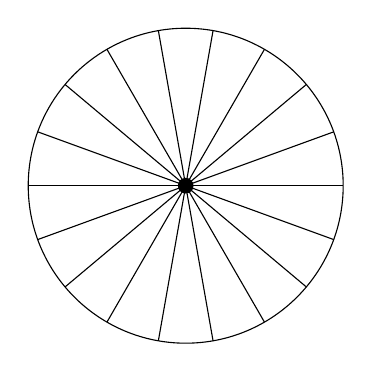
\begin{tikzpicture}
    \draw (0,0) circle (2cm);
    \foreach \x in {0,20,...,350}
    \draw[\OPTblue] (0,0) -- (\x:2cm);
    \node[\OPTblue,circle,fill,inner sep=2pt] (hub) at (0,0) {};
  \end{tikzpicture}
  \caption{由一个中心与辐条组成的二维圆盘}
  \label{fig:hub-and-spokes}
\end{figure}

我们可以利用这一思想来表达包含 $n$ 维路径构造器的高阶归纳类型,其中 $n>1$,而这些构造器仅包含一维路径构造器。
关键在于,我们可以通过一个 $(n-1)$ 维对象参数化的连续的一维路径族来获得一个 $n$ 维路径。
最简单的 $(n-1)$ 维对象是 $(n-1)$ 球面,尽管在某些情况下,一个不同的对象可能更合适。
(回顾一下,我们能够在 \cref{sec:suspension} 中使用悬挂 (suspensions) 递归地定义球面,这仅涉及一维路径构造器。
事实上,悬挂也可以看作是这种思想的一个实例,因为它涉及一个由被悬挂的类型参数化的一维路径族。)

\index{圆环}
例如,前一节中的圆环 $T^2$ 可以通过以下方式生成:
\begin{itemize}
  \item 一个点 $b:T^2$,
  \item 一条路径 $p:b=b$,
  \item 另一条路径 $q:b=b$,
  \item 一个点 $h:T^2$, 以及
  \item 对每个 $x:\Sn^1$,一条路径 $s(x) : f(x)=h$,其中 $f:\Sn^1\to T^2$ 定义为 $f(\base)\defeq b$ 和 $\ap f \lloop \defid p \ct q \ct \opp p \ct \opp q$。
\end{itemize}
这个版本的圆环的归纳原理表明,给定 $P:T^2\to\type$,对于截面 $\prd{x:T^2} P(x)$,我们需要
\begin{itemize}
  \item 一个点 $b':P(b)$,
  \item 一条路径 $p' : \dpath P p {b'} {b'}$,
  \item 一条路径 $q' : \dpath P q {b'} {b'}$,
  \item 一个点 $h':P(h)$, 以及
  \item 对每个 $x:\Sn^1$,一条路径 $\dpath {P}{s(x)}{g(x)}{h'}$,其中 $g:\prd{x:\Sn^1} P(f(x))$ 定义为 $g(\base)\defeq b'$ 和 $\apd g \lloop \defid t(p' \ct q' \ct \opp{(p')} \ct \opp{(q')})$。
  在后者中,$\ct$ 表示依赖路径的连接,$t:\eqv{(\dpath{P}{\ap f \lloop}{b'}{b'})}{(\dpath{P\circ f}{\lloop}{b'}{b'})}$ 的定义留给读者完成。
\end{itemize}
注意,不需要依赖 2-路径或 $\apdtwofunc{}$。
我们将计算规则的书写留给读者。

\begin{rmk}\label{rmk:spokes-no-hub}
有人可能会质疑引入中心点 $h$ 的必要性;为什么我们不能简单地添加连续连接圆盘边界到边界上某个点的路径,如 \cref{fig:spokes-no-hub} 所示?
然而,这在没有进一步修改的情况下是行不通的。
因为,如果给定某个 $f:\Sn^1 \to X$,我们给出一个路径构造器连接每个 $f(x)$ 到 $f(\base)$,那么我们最终得到的更像是 \cref{fig:spokes-no-hub-ii} 中的图像,一个顶点被扭曲并粘合到其底部某个点上的锥体。
问题在于,从 $f(\base)$ 到其本身的指定路径可能不是反身性 (reflexivity)。
我们可以通过添加一个 2-维路径构造器来解决这个问题,以确保这种情况,但使用一个独立的中心避免了需要任何维度超过 1 的路径构造器。
\end{rmk}

\begin{figure}
  \centering
  \begin{minipage}{2in}
    \begin{center}
      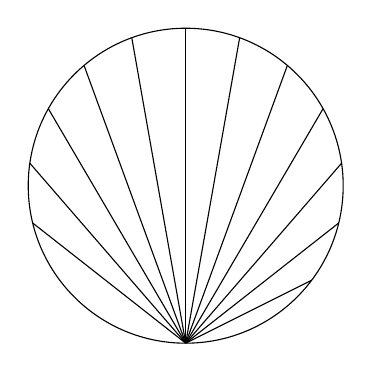
\begin{tikzpicture}
        \draw (0,0) circle (2cm);
        \clip (0,0) circle (2cm);
        \foreach \x in {0,15,...,165}
        \draw[\OPTblue] (0,-2cm) -- (\x:4cm);
      \end{tikzpicture}
    \end{center}
    \caption{无中心的辐条}
    \label{fig:spokes-no-hub}
  \end{minipage}
  \qquad
  \begin{minipage}{2in}
    \begin{center}
      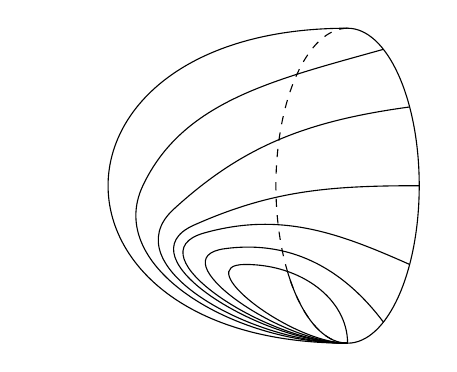
\begin{tikzpicture}[xscale=1.3]
        \draw (0,0) arc (-90:90:.7cm and 2cm) ;
        \draw[dashed] (0,4cm) arc (90:270:.7cm and 2cm) ;
        \draw[\OPTblue] (0,0) to[out=90,in=0] (-1,1) to[out=180,in=180] (0,0);
        \draw[\OPTblue] (0,4cm) to[out=180,in=180,looseness=2] (0,0);
        \path (0,0) arc (-90:-60:.7cm and 2cm) node (a) {};
        \draw[\OPTblue] (a.center) to[out=120,in=10] (-1.2,1.2) to[out=190,in=180] (0,0);
        \path (0,0) arc (-90:-30:.7cm and 2cm) node (b) {};
        \draw[\OPTblue] (b.center) to[out=150,in=20] (-1.4,1.4) to[out=200,in=180] (0,0);
        \path (0,0) arc (-90:0:.7cm and 2cm) node (c) {};
        \draw[\OPTblue] (c.center) to[out=180,in=30] (-1.5,1.5) to[out=210,in=180] (0,0);
        \path (0,0) arc (-90:30:.7cm and 2cm) node (d) {};
        \draw[\OPTblue] (d.center) to[out=190,in=50] (-1.7,1.7) to[out=230,in=180] (0,0);
        \path (0,0) arc (-90:60:.7cm and 2cm) node (e) {};
        \draw[\OPTblue] (e.center) to[out=200,in=70] (-2,2) to[out=250,in=180] (0,0);
        \clip (0,0) to[out=90,in=0] (-1,1) to[out=180,in=180] (0,0);
        \draw (0,4cm) arc (90:270:.7cm and 2cm) ;
      \end{tikzpicture}
    \end{center}
    \caption{无中心的辐条 II}
    \label{fig:spokes-no-hub-ii}
  \end{minipage}
\end{figure}

\begin{rmk}
  \index{计算规则!命题的}%
  请注意,这种将高阶路径转换为一阶路径的方法并不保留这些路径的判断计算规则,但它确实保留了命题计算规则。
\end{rmk}

\index{胞腔复形|)}%
\index{CW 复形|)}%

\index{中心与辐条|)}%


\section{推挤 (Pushouts)}
\label{sec:colimits}

\index{类型!极限}%
\index{类型!余极限}%
\index{极限!类型的极限}%
\index{余极限!类型的余极限}%
从范畴论 (category-theoretic) 的角度来看,任何基础系统的一个重要方面是构造极限 (limits) 和余极限 (colimits) 的能力。
在集合论基础中,这些是集合的极限和余极限,而在我们的情况下,它们是\emph{类型 (types)}的极限和余极限。
我们在 \cref{sec:universal-properties} 中已经看到,笛卡尔乘积类型具有类型范畴积 (categorical product of types) 的正确通用性质 (universal property),而在 \cref{ex:coprod-ump} 中,余积类型 (coproduct types) 也具有它们预期的通用性质。

如 \cref{sec:universal-properties} 中所述,可以使用等式类型 (identity types) 和 $\Sigma$ 类型来构造更一般的极限,例如 $f:A\to C$ 和 $g:B\to C$ 的纤维积 (pullback)\index{纤维积} 是 $\sm{a:A}{b:B} (f(a)=g(b))$(见 \cref{ex:pullback})。
然而,更一般的\emph{余极限}需要识别来自不同类型的元素,高阶归纳类型 (higher inductive types) 对此非常适用。
由于我们所有的构造都是同伦不变的 (homotopy-invariant),因此我们所有的余极限都是\emph{同伦余极限 (homotopy colimits)},但为了简洁起见,我们省略了无处不在的形容词。

本节我们讨论\emph{推挤 (pushouts)},作为也许最简单且最有用的余极限之一。
确实,人们期望所有有限余极限(对于一个合适的同伦定义“有限”)可以通过推挤和有限余积构造。
也可以使用高阶归纳类型直接构造更一般的余极限,但这有些技术性问题,并且不完全令人满意,因为我们尚未有一个完全通用的同伦一致图的良好概念。

\indexsee{类型!推挤}{推挤}%
\index{推挤|(defstyle}%
\index{跨 (span)}%
假设给定一个类型和函数的跨图:
\[\Ddiag=\;\vcenter{\xymatrix{C \ar^g[r] \ar_f[d] & B \\ A & }}\]
该跨图的\define{推挤 (pushout)} 是高阶归纳类型 $A\sqcup^CB$,由以下内容呈现:
\begin{itemize}
  \item 一个函数 $\inl:A\to A\sqcup^CB$,
  \item 一个函数 $\inr:B \to A\sqcup^CB$, 以及
  \item 对于每个 $c:C$,一个路径 $\glue(c):(\inl(f(c))=\inr(g(c)))$。
\end{itemize}
换句话说,$A\sqcup^CB$ 是 $A$ 和 $B$ 的不交并 (disjoint union),并且对于每个 $c:C$,有一个 $f(c)$ 和 $g(c)$ 相等的证据。
递归原理 (recursion principle) 表示,如果 $D$ 是另一个类型,我们可以通过定义以下内容来定义一个映射 $s:A\sqcup^CB\to{}D$:
\begin{itemize}
  \item 对于每个 $a:A$,$s(\inl(a))$ 的值:$D$,
  \item 对于每个 $b:B$,$s(\inr(b))$ 的值:$D$,以及
  \item 对于每个 $c:C$,$\mapfunc{s}(\glue(c))$ 的值:$s(\inl(f(c)))=s(\inr(g(c)))$。
\end{itemize}
我们将归纳原理的表述留给读者。
它还暗示了唯一性原理 (uniqueness principle),即如果 $s,s':A\sqcup^CB\to{}D$ 是两个映射,并且
\index{唯一性原理!推挤上函数的命题唯一性原理}%
\begin{align*}
  s(\inl(a))&=s'(\inl(a))\\
  s(\inr(b))&=s'(\inr(b))\\
  \mapfunc{s}(\glue(c))&=\mapfunc{s'}(\glue(c))
  \qquad\text{(基于前两个等式)}
\end{align*}
对于每个 $a,b,c$,则 $s=s'$。

为了表述推挤的通用性质 (universal property),我们引入以下定义。

\begin{defn}\label{defn:cocone}
给定一个跨图 $\Ddiag= (A \xleftarrow{f} C \xrightarrow{g} B)$ 和一个类型 $D$,在 $\Ddiag$ 下,顶点为 $D$ 的\define{余锥 (cocone)}\indexdef{余锥}%
\index{余锥的顶点}%
由函数 $i:A\to{}D$ 和 $j:B\to{}D$ 以及同伦 $h : \prd{c:C} (i(f(c))=j(g(c)))$ 组成:
\[\uppercurveobject{{ }}\lowercurveobject{{ }}\twocellhead{{ }}
\xymatrix{C \ar^g[r] \ar_f[d] \drtwocell{^h} & B \ar^j[d] \\ A \ar_i[r] & D
}\]
我们用 $\cocone{\Ddiag}{D}$ 表示所有此类余锥的类型,即
\[ \cocone{\Ddiag}{D} \defeq
\sm{i:A\to D}{j:B\to D} \prd{c:C} (i(f(c))=j(g(c))).
\]
\end{defn}

当然,存在一个在 $\Ddiag$ 下,顶点为 $A\sqcup^C B$ 的标准余锥,由 $\inl$、$\inr$ 和 $\glue$ 组成。
\[\uppercurveobject{{ }}\lowercurveobject{{ }}\twocellhead{{ }}
\xymatrix{C \ar^g[r] \ar_f[d] \drtwocell{^\glue\ \ } & B \ar^\inr[d] \\
A \ar_-\inl[r] & A\sqcup^CB }\]
以下引理表明这是通用的此类余锥。

\begin{lem}\label{thm:pushout-ump}
\index{通用性质!推挤的通用性质}%
对于任何类型 $E$,存在等价
\[ (A\sqcup^C B \to E) \;\eqvsym\; \cocone{\Ddiag}{E}. \]
\end{lem}
\begin{proof}
  我们考虑任意类型 $E:\type$。
  存在一个标准函数 $c_\sqcup$,定义如下
  \[\function{(A\sqcup^CB\to{}E)}{\cocone{\Ddiag}{E}}
  {t}{(t\circ{}\inl,t\circ{}\inr,\mapfunc{t}\circ{}\glue)}\]
  我们用非正式符号 $t\mapsto\composecocone{t}c_\sqcup$ 表示此函数。
  我们证明这是一个等价。

  首先,给定 $c=(i,j,h):\cocone{\mathscr{D}}{E}$,我们需要构造一个
  从 $A\sqcup^CB$ 到 $E$ 的映射 $\mathsf{s}(c)$。
  \[\uppercurveobject{{ }}\lowercurveobject{{ }}\twocellhead{{ }}
  \xymatrix{C \ar^g[r] \ar_f[d] \drtwocell{^h} & B \ar^{j}[d] \\
  A \ar_-{i}[r] & E }\]
  映射 $\mathsf{s}(c)$ 定义如下:
  \begin{align*}
    \mathsf{s}(c)(\inl(a))&\defeq i(a),\\
    \mathsf{s}(c)(\inr(b))&\defeq j(b),\\
    \mapfunc{\mathsf{s}(c)}(\glue(x))&\defid h(x)。
  \end{align*}
  我们定义了一个映射
  \[\function{\cocone{\Ddiag}{E}}{(A\sqcup^CB\to{}E)}{c}{\mathsf{s}(c)}\]
  我们需要证明此映射是 $t\mapsto{}\composecocone{t}c_\sqcup$ 的逆映射。
  一方面,如果 $c=(i,j,h):\cocone{\Ddiag}{E}$,我们有
  \begin{align*}
    \composecocone{\mathsf{s}(c)}c_\sqcup & =
    (\mathsf{s}(c)\circ\inl,\mathsf{s}(c)\circ\inr,
    \mapfunc{\mathsf{s}(c)}\circ\glue) \\
    & = (\lamu{a:A} \mathsf{s}(c)(\inl(a)),\;
    \lamu{b:B} \mathsf{s}(c)(\inr(b)),\;
    \lamu{x:C} \mapfunc{\mathsf{s}(c)}(\glue(x))) \\
    & = (\lamu{a:A} i(a),\;
    \lamu{b:B} j(b),\;
    \lamu{x:C} h(x)) \\
    & \jdeq (i, j, h) \\
    & = c。
  \end{align*}
%
  另一方面,如果 $t:A\sqcup^CB\to{}E$,我们想证明
  $\mathsf{s}(\composecocone{t}c_\sqcup)=t$。
  对于 $a:A$,我们有
  \[\mathsf{s}(\composecocone{t}c_\sqcup)(\inl(a))=t(\inl(a))\]
  因为 $\composecocone{t}c_\sqcup$ 的第一个分量是 $t\circ\inl$。以
  同样的方式,对于 $b:B$,我们有
  \[\mathsf{s}(\composecocone{t}c_\sqcup)(\inr(b))=t(\inr(b))\]
  对于 $x:C$,我们有
  \[\mapfunc{\mathsf{s}(\composecocone{t}c_\sqcup)}(\glue(x))
  =\mapfunc{t}(\glue(x))\]
  因此 $\mathsf{s}(\composecocone{t}c_\sqcup)=t$。

  这证明了 $c\mapsto\mathsf{s}(c)$ 是 $t\mapsto{}\composecocone{t}c_\sqcup$ 的准逆映射,正如所需。
\end{proof}

许多标准的同伦理论构造可以表示为(同伦)推挤。
\begin{itemize}
  \item 跨图 $\unit \leftarrow A \to \unit$ 的推挤是 \define{悬挂 (suspension)} $\susp A$(见 \cref{sec:suspension})。%
  \index{悬挂}
  \symlabel{join}
  \item $A \xleftarrow{\proj1} A\times B \xrightarrow{\proj2} B$ 的推挤称为 $A$ 和 $B$ 的\define{连接 (join)},记为 $A*B$。%
  \indexdef{连接!类型的连接}
  \item $\unit \leftarrow A \xrightarrow{f} B$ 的推挤称为 $f$ 的\define{锥体 (cone)}或\define{余纤维 (cofiber)}。%
  \indexdef{锥体!函数的锥体}%
  \indexsee{映射锥体}{函数的锥体}%
  \indexdef{余纤维}
  \symlabel{wedge}
  \item 如果 $A$ 和 $B$ 具有基点 (basepoints) $a_0:A$ 和 $b_0:B$,则 $A \xleftarrow{a_0} \unit \xrightarrow{b_0} B$ 的推挤是\define{楔积 (wedge)} $A\vee B$。%
  \indexdef{楔积}
  \symlabel{smash}
  \item 如果 $A$ 和 $B$ 是如前所述的有基点类型,则定义 $f:A\vee B \to A\times B$ 为 $f(\inl(a))\defeq (a,b_0)$ 和 $f(\inr(b))\defeq (a_0,b)$,其中 $\ap f \glue \defid \refl{(a_0,b_0)}$。
  那么 $f$ 的锥体称为\define{劈积 (smash product)} $A\wedge B$。%
  \indexdef{劈积}
\end{itemize}
我们将在 \cref{cha:hlevels,cha:homotopy} 中进一步讨论推挤。

\begin{rmk}
  正如在 \cref{subsec:prop-trunc} 中所述,对于有基点的空间,劈积和楔积的符号 $\wedge$ 和 $\vee$ 也用于逻辑中的“与 (and)”和“或 (or)”。
  由于同伦类型论中的类型既可以表现得像空间,也可以表现得像命题,因此存在冲突的潜在可能性——但由于它们很少同时这样做,通常上下文可以消除歧义。
  此外,劈积和楔积仅适用于\emph{有基点}的空间,而唯一的有基点的纯命题是 $\top\jdeq\unit$——并且我们有 $\unit\wedge \unit = \unit$ 和 $\unit\vee\unit=\unit$ 对于 $\wedge$ 和 $\vee$ 的任何含义都成立。
\end{rmk}

\index{推挤|)}%

\begin{rmk}
  请注意,余极限通常不保留截断性 (truncatedness)。
  例如,$\Sn^0$ 和 \unit 都是集合 (sets),但 $\unit \leftarrow \Sn^0 \to \unit$ 的推挤是 $\Sn^1$,它不是集合。
  因此,如果我们对 $n$-类型范畴 (category of $n$-types) 中的余极限感兴趣(特别是在集合的范畴中),我们需要以某种方式“截断”余极限。
  我们将在 \cref{sec:hittruncations,cha:hlevels,cha:set-math} 中回到这一点。
\end{rmk}

\section{截断 (Truncations)}
\label{sec:hittruncations}

\index{截断!命题截断|(propositional truncation|(}%
在\cref{subsec:prop-trunc}中,我们介绍了命题截断 (propositional truncation) 作为一种新的类型构造操作;现在我们发现它可以作为高阶归纳类型 (higher inductive types) 的一种特殊情况来获得。这将理解截断的问题简化为理解高阶归纳类型的问题,而高阶归纳类型至少是可以系统处理的。这个现象也很有趣,因为它为我们提供了第一个真正\emph{递归 (recursive)} 的高阶归纳类型的例子,即它的构造器从正在定义的类型中获取输入(就像后继 $\suc:\nat\to\nat$ 一样)。

设 $A$ 是一个类型;我们定义其命题截断 $\brck A$ 为由以下构造器生成的高阶归纳类型:
\begin{itemize}
  \item 一个函数 $\bprojf : A \to \brck A$,以及
  \item 对于每个 $x,y:\brck A$,一个路径 $x=y$。
\end{itemize}
请注意,第二个构造器实际上是断言 $\brck A$ 是一个纯命题 (mere proposition)。因此,$\brck A$ 的定义可以解释为 $\brck A$ 是由 $A\to\brck A$ 的函数和它是一个纯命题的事实自由生成的。

该高阶归纳定义的递归原理 (recursion principle) 很容易写出来:它表示给定任意类型 $B$,以及
\begin{itemize}
  \item 一个函数 $g:A\to B$,以及
  \item 对于任意 $x,y:B$,一个路径 $x=_B y$,
\end{itemize}
存在一个函数 $f:\brck A \to B$ 使得
\begin{itemize}
  \item 对于所有 $a:A$,$f(\bproj a) \jdeq g(a)$,以及
  \item 对于任意 $x,y:\brck A$,函数 $\apfunc f$ 将 $\brck A$ 中指定的路径 $x=y$ 映射到 $B$ 中指定的路径 $f(x) = f(y)$(命题性地)。
\end{itemize}
\index{递归原理!截断的递归原理}%
这些正是我们在\cref{subsec:prop-trunc}中为命题截断的递归原理所陈述的假设——一个 $A\to B$ 的函数,且 $B$ 是一个纯命题——结论的第一部分正是我们在那里陈述的内容。结论的第二部分($\apfunc f$ 的作用)之前没有提到,但在这种情况下是空洞的,因为 $B$ 是一个纯命题,所以\emph{任何}两条路径在其中都自动相等。

\index{归纳原理!截断的归纳原理}%
$\brck A$ 还有一个归纳原理 (induction principle),它表示给定任意 $B:\brck A \to \type$ 以及
\begin{itemize}
  \item 一个函数 $g:\prd{a:A} B(\bproj a)$,以及
  \item 对于任意 $x,y:\brck A$ 和 $u:B(x)$ 以及 $v:B(y)$,一个依赖路径 $q:\dpath{B}{p(x,y)}{u}{v}$,其中 $p(x,y)$ 是从 $\brck A$ 的第二个构造器中获得的路径,
\end{itemize}
存在 $f:\prd{x:\brck A} B(x)$ 使得 $f(\bproj a)\jdeq g(a)$ 对于 $a:A$ 成立,并且还有另一个计算规则。然而,由于在任何两个纯命题之间至多可以存在一个函数(最多到同伦),这个归纳原理并没有太大用处(参见\cref{ex:prop-trunc-ind})。

\index{截断!命题截断|)}%
\index{截断!集合|(set truncation|)}%

\index{集合|(set|(}%
我们可以扩展这个想法来构造类似的截断,落在 $n$-类型中,对于任意 $n$。例如,我们可以定义\emph{0-截断 (0-truncation)} $\trunc0A$ 为由以下内容生成的:
\begin{itemize}
  \item 一个函数 $\tprojf0 : A \to \trunc0 A$,以及
  \item 对于每个 $x,y:\trunc0A$ 和每个 $p,q:x=y$,一个路径 $p=q$。
\end{itemize}
然后 $\trunc0A$ 将由一个 $A\to \trunc0A$ 的函数以及 $\trunc0A$ 是一个集合 (set) 的断言自由生成。它的一个自然的归纳原理表示,给定 $B:\trunc0 A \to \type$ 以及
\begin{itemize}
  \item 一个函数 $g:\prd{a:A} B(\tproj0a)$,以及
  \item 对于任意 $x,y:\trunc0A$,以及 $z:B(x)$ 和 $w:B(y)$,以及每个 $p,q:x=y$ 和 $r:\dpath{B}{p}{z}{w}$ 以及 $s:\dpath{B}{q}{z}{w}$,一个 $v:\dpath{\dpath{B}{-}{z}{w}}{u(x,y,p,q)}{r}{s}$ 的2路径,其中 $u(x,y,p,q):p=q$ 是从 $\trunc0A$ 的第二个构造器中获得的,
\end{itemize}
存在 $f:\prd{x:\trunc0A} B(x)$ 使得 $f(\tproj0a)\jdeq g(a)$ 对于所有 $a:A$ 成立,并且 $\apdtwo{f}{u(x,y,p,q)}$ 是上面指定的2路径。(如同命题情况,后者的条件被证明是不太重要的。)然而,从这可以证明一个更有用的归纳原理。

\begin{lem}\label{thm:trunc0-ind}
假设给定 $B:\trunc0 A \to \type$ 以及 $g:\prd{a:A} B(\tproj0a)$,并假设每个 $B(x)$ 是一个集合。然后存在 $f:\prd{x:\trunc0A} B(x)$ 使得 $f(\tproj0a)\jdeq g(a)$ 对于所有 $a:A$ 成立。
\end{lem}
\begin{proof}
  只需为上述的任意 $x,y,z,w,p,q,r,s$ 构造一个2路径 $v:\dpath{B}{u(x,y,p,q)}{r}{s}$ 即可。然而,根据依赖2路径的定义,这只是 $B(y)$ 中的一个普通2路径。由于 $B(y)$ 是一个集合,因此在任何两个平行路径之间都存在一个2路径。
\end{proof}

这暗示了预期的通用性质。

\begin{lem}\label{thm:trunc0-lump}
\index{通用性质!截断的通用性质}%
对于任意集合 $B$ 和任意类型 $A$,与 $\tprojf0:A\to \trunc0A$ 组合的合成决定了一个等价
\[ \eqvspaced{(\trunc0A\to B)}{(A\to B)}。 \]
\end{lem}
\begin{proof}
  当 $B$ 是常数族时,\cref{thm:trunc0-ind} 的特例提供了一个从右到左的映射,它是从左到右的“与 $\tprojf0$ 组合”函数的右逆。
  要证明它也是左逆,设 $h:\trunc0A\to B$,并通过将\cref{thm:trunc0-ind} 应用于复合 $a\mapsto h(\tproj0a)$ 来定义 $h':\trunc0A\to B$。因此,对于任意 $a:A$,$h'(\tproj0a)=h(\tproj0a)$。

  然而,由于 $B$ 是一个集合,对于任意 $x:\trunc0A$,类型 $h(x)=h'(x)$ 是一个纯命题,因此也是一个集合。因此,依据\cref{thm:trunc0-ind},观察到 $h'(\tproj0a)=h(\tproj0a)$ 对于任意 $a:A$ 表明对于任意 $x:\trunc0A$,$h(x)=h'(x)$,因此 $h=h'$。
\end{proof}

\index{集合的极限}%
\index{集合的余极限}%
例如,这使我们能够构造集合的余极限。我们已经看到,如果 $A \xleftarrow{f} C \xrightarrow{g} B$ 是一组集合,则推挤 $A\sqcup^C B$ 可能不再是一个集合。(例如,如果 $A$ 和 $B$ 是 \unit 而 $C$ 是 \bool,则推挤是 $\Sn^1$。)然而,我们可以通过截断构造一个集合的推挤,并具有与其他集合相关的预期通用性质。

\begin{lem}\label{thm:set-pushout}
\index{通用性质!推挤的通用性质}%
设 $A \xleftarrow{f} C \xrightarrow{g} B$ 是一组集合。则对于任意集合 $E$,存在一个典型的等价
\[ \Parens{\trunc0{A\sqcup^C B} \to E} \;\eqvsym\; \cocone{\Ddiag}{E}。 \]
\end{lem}
\begin{proof}
  结合\cref{thm:pushout-ump,thm:trunc0-lump} 中的等价性。
\end{proof}

我们将 $\trunc0{A\sqcup^C B}$ 称为\define{集合推挤 (set-pushout)}%
\indexdef{集合推挤}%
\index{推挤!集合的推挤}的 $f$ 和 $g$,以将其与(同伦)推挤 $A\sqcup^C B$ 区分开来。或者,我们可以直接修改\cref{sec:colimits} 中的推挤定义,以包括0截断构造器,从而避免事后截断。类似的备注也适用于任何类型的集合余极限;我们将在\cref{cha:set-math} 中进一步探讨这个问题。

然而,虽然上述的0截断定义是可行的——它给出了我们想要的结果,并且是一致的——它有几个问题。首先,它不太适合高阶归纳类型的一般理论。通常,直接处理像我们为 $\trunc0A$ 给出的第二个构造器这样的构造器是很棘手的,因为它们的\emph{输入}不仅涉及正在定义的类型中的元素,还涉及其中的路径。

然而,这个问题可以相当容易地解决。回想一下,在\cref{sec:bool-nat} 中我们提到,我们可以通过让构造器获取一个类型 $W$ 的归纳类型 $W$ 的“无限多的参数”,从而允许一个构造器接受无限多个 $W$ 类型的参数,例如通过让它获取类型 $\nat\to W$ 的单个参数。这背后有一个普遍的原则:为了模拟具有奇特输入的构造器,使用辅助归纳类型(如 \nat)对它们进行参数化,将输入简化为具有归纳域的简单函数。

对于0截断,我们可以考虑辅助的\emph{高阶}归纳类型 $S$,它由两个点 $a,b:S$ 和两条路径 $p,q:a=b$ 生成。然后,$\trunc 0A$ 中看似奇怪的构造器可以被替换为无可非议的
\begin{itemize}
  \item 对于每个 $f:S\to \trunc 0A$,一条路径 $\apfunc{f}(p) = \apfunc{f}(q)$。
\end{itemize}
因为给定 $S$ 的映射等同于给出两个点和它们之间的两条平行路径,这将产生相同的归纳原理。

\index{集合|)}%

\index{截断!集合截断|)}%
\index{截断!n-截断@$n$-截断}%
然而,我们当前的0截断定义的一个更严重的问题是,它不能很好地推广。如果我们想描述一个统一定义的“$n$-截断”到 $n$-类型中的概念,对于任意 $n:\nat$,那么这种方法是不可行的,因为第二个构造器需要的参数数量随着 $n$ 的增加而增加。因此,在\cref{sec:truncations} 中,我们将使用一个不同的想法来构造这些,基于一个观察,即上述引入的类型 $S$ 等价于圆 $\Sn^1$。这包括了0截断作为一个特殊情况,并满足\cref{thm:trunc0-ind,thm:trunc0-lump} 的广义版本。


\section{商 (Quotients)}
\label{sec:set-quotients}

集合的一种特别重要的余极限是通过关系的\emph{商 (quotient)}。也就是说,设 $A$ 是一个集合,$R:A\times A \to \prop$ 是一族纯命题(\define{纯关系 (mere relation)})。\indexdef{关系!纯关系}%
\indexdef{纯关系}%
它的商应该是以下两个投影的集合并等化子 (set-coequalizer)
\[ \tsm{a,b:A} R(a,b) \rightrightarrows A。 \]
我们也可以直接描述它,作为由以下内容生成的高阶归纳类型 $A/R$:
\index{集合商|(defstyle}%
\indexsee{集合的商}{集合商}%
\indexsee{类型的商}{集合商}%
\begin{itemize}
  \item 一个函数 $q:A\to A/R$;
  \item 对于每个 $a,b:A$,如果 $R(a,b)$,则有一个等式 $q(a)=q(b)$;以及
  \item 0截断构造器:对于所有 $x,y:A/R$ 和 $r,s:x=y$,我们有 $r=s$。
\end{itemize}
我们有时会将这个高阶归纳类型 $A/R$ 称为 $A$ 关于 $R$ 的\define{集合商},以强调它按定义生成了一个集合。(在同伦理论中有更一般的“商”概念,但它们大多超出了本书的范围。然而,在\cref{sec:rezk} 中,我们将考虑一个类型关于1-群胚 (1-groupoid) 的“商”,这是集合商之上的下一个层次。)

\begin{rmk}\label{rmk:quotient-of-non-set}
事实上,定义集合商时,并不需要 $A$ 是一个集合。尽管如此,这通常是最感兴趣的情况。
\end{rmk}

\begin{lem}\label{thm:quotient-surjective}
函数 $q:A\to A/R$ 是满射。
\end{lem}
\begin{proof}
  我们必须证明,对于任意 $x:A/R$,存在一个 $a:A$ 使得 $q(a)=x$。我们使用 $A/R$ 的归纳原理。第一个情况是显然的:如果 $x$ 是 $q(a)$,那么当然存在一个 $a$,使得 $q(a)=q(a)$。由于目标是一个纯命题,它自动尊重所有路径构造器,因此我们完成了证明。
\end{proof}

现在我们可以证明集合商具有预期的集合并等化子的通用性质。

\begin{lem}\label{thm:quotient-ump}
对于任意集合 $B$,预合成 $q$ 得到一个等价
\[ \eqvspaced{(A/R \to B)}{\Parens{\sm{f:A\to B} \prd{a,b:A} R(a,b) \to (f(a)=f(b))}}。 \]
\end{lem}
\begin{proof}
  从右到左的 $\blank\circ q$ 的准逆是 $A/R$ 的递归原理。也就是说,给定 $f:A\to B$,使得
  \narrowequation{\prd{a,b:A} R(a,b) \to (f(a)=f(b)),} 我们通过定义 $\bar f:A/R\to B$ 为 $\bar f(q(a))\defeq f(a)$。
  这个定义等式正好说明了 $(f\mapsto \bar f)$ 是 $(\blank\circ q)$ 的右逆。

  为了证明它也是左逆,我们必须证明,对于任意 $g:A/R\to B$ 和 $x:A/R$,我们有 $g(x) = \overline{g\circ q}(x)$。
  然而,根据\cref{thm:quotient-surjective},仅存在一个 $a$ 使得 $q(a)=x$。由于我们想要的等式是一个纯命题,我们可以假设确实存在这样的 $a$,在这种情况下,$g(x) = g(q(a)) = \overline{g\circ q}(q(a)) = \overline{g\circ q}(x)$。
\end{proof}

当然,经典情况下通常考虑 $R$ 是一个\define{等价关系 (equivalence relation)},即我们有
\indexdef{关系!等价}%
\indexsee{等价!关系}{关系, 等价}%
%
\begin{itemize}
  \item \define{自反性 (reflexivity)}:$\prd{a:A} R(a,a)$,
  \indexdef{自反性!关系的自反性}%
  \indexdef{关系!自反性}%
  \item \define{对称性 (symmetry)}:$\prd{a,b:A} R(a,b) \to R(b,a)$,以及
  \indexdef{对称性!关系的对称性}%
  \indexdef{关系!对称性}%
  \item \define{传递性 (transitivity)}:$\prd{a,b,c:C} R(a,b) \times R(b,c) \to R(a,c)$。
  \indexdef{传递性!关系的传递性}%
  \indexdef{关系!传递性}%
\end{itemize}
%
在这种情况下,集合商 $A/R$ 具有额外的良好性质,正如我们将在\cref{sec:piw-pretopos} 中看到的:例如,我们有 $R(a,b) \eqvsym (\id[A/R]{q(a)}{q(b)})$。
\symlabel{等价关系}
我们通常将等价关系 $R(a,b)$ 以中缀形式写为 $a\eqr b$。

等价关系的商也可以通过其他方式构造。集合论的方法是将等价类视为幂集\index{幂集} $A$ 的子集。我们也可以在类型论中模仿这种“泛型 (impredicative)”构造。
\index{泛型!商}

\begin{defn}
  如果对于任意 $b:A$ 我们有 $\eqv{R(a,b)}{P(b)}$,则谓词 $P:A\to\prop$ 是关系 $R : A \times A \to \prop$ 的\define{等价类 (equivalence class)}。
\end{defn}

由于 $R$ 和 $P$ 是纯命题,等价 $\eqv{R(a,b)}{P(b)}$ 等同于蕴涵 $R(a,b) \to P(b)$ 和 $P(b) \to R(a,b)$。当然,对于任意 $a:A$,我们有规范的等价类 $P_a(b) \defeq R(a,b)$。

\begin{defn}\label{def:VVquotient}
我们定义
\begin{equation*}
  A\sslash R \defeq \setof{ P:A\to\prop | P \text{ 是 } R \text{ 的一个等价类}}。
\end{equation*}
函数 $q':A\to A\sslash R$ 定义为 $q'(a) \defeq P_a$。
\end{defn}

\begin{thm}
  对于任意集合 $A$ 上的等价关系 $R$,类型 $A\sslash R$ 与集合商 $A/R$ 等价。
\end{thm}
\begin{proof}
  首先注意,如果 $R(a,b)$,则由于 $R$ 是等价关系,对于任意 $c:A$,我们有 $R(a,c) \Leftrightarrow R(b,c)$。因此,通过一值性 (univalence),$R(a,c) = R(b,c)$,因此通过函数扩展性 (function extensionality),$P_a=P_b$,即 $q'(a)=q'(b)$。因此,根据\cref{thm:quotient-ump},我们有一个从 $A/R$ 到 $A\sslash R$ 的诱导映射 $f$,使得 $f\circ q = q'$。

  我们证明 $f$ 是单射且满射,因此是一个等价。满射性直接来自 $q'$ 的满射性,后者本质上是由 $A\sslash R$ 的定义决定的。对于单射性,如果 $f(x)=f(y)$,则为了证明纯命题 $x=y$,通过 $q$ 的满射性,我们可以假设 $x=q(a)$ 和 $y=q(b)$ 对于某些 $a,b:A$。然后,对于任意 $c:A$,$R(a,c) = f(q(a))(c) = f(q(b))(c) = R(b,c)$,特别地,$R(a,b) = R(b,b)$。但是 $R(b,b)$ 是有元素的,因为 $R$ 是等价关系,因此 $R(a,b)$ 也是有元素的。因此 $q(a)=q(b)$,因此 $x=y$。
\end{proof}

在\cref{subsec:quotients} 中,我们将给出该定理的另一种证明。注意,与 $A/R$ 不同,构造 $A\sslash R$ 提升了宇宙层次:如果 $A:\UU_i$ 且 $R:A\to A\to \prop_{\UU_i}$,则在 $A\sslash R$ 的定义中,我们还必须使用 $\prop_{\UU_i}$ 来包含所有等价类,因此 $A\sslash R : \UU_{i+1}$。当然,如果我们假设来自\cref{subsec:prop-subsets} 的命题重缩放公理 (propositional resizing axiom),我们可以避免这个问题。

\begin{rmk}\label{defn-Z}
之前的两个构造提供了普遍的商,但在特殊情况下,可能存在更简单的构造。例如,我们可以定义整数 \Z 作为集合商
\indexdef{整数}%
\indexdef{数字!整数}%
%
\[ \Z \defeq (\N \times \N)/{\eqr} \]
%
其中 $\eqr$ 是通过以下方式定义的等价关系:
%
\[ (a,b) \eqr (c,d) \defeq (a + d = b + c)。 \]
%
换句话说,一个对 $(a,b)$ 代表整数 $a - b$。然而,在这种情况下存在\emph{规范的代表 (canonical representatives)}:即形如 $(n,0)$ 或 $(0,n)$ 的代表。
\end{rmk}

以下引理表明,当出现这种情况时,我们不需要任一一般商的构造。(一个函数 $r:A\to A$ 称为\define{幂等的 (idempotent)}%
\indexdef{函数!幂等的}%
\indexdef{幂等的!函数}%
当且仅当 $r\circ r = r$。)

\begin{lem}\label{lem:quotient-when-canonical-representatives}
假设 $\eqr$ 是集合 $A$ 上的关系,并且存在一个幂等 $r:A \to A$,使得对于所有 $x,y: A$,$\eqv{(r(x) = r(y))}{(x \eqr y)}$。(这意味着 $\eqr$ 是一个等价关系。)那么类型
%
\begin{equation*}
(A/{\eqr}) \defeq \Parens{\sm{x : A} r(x) = x}
\end{equation*}
%
满足 $A$ 关于 $\eqr$ 的集合商的通用性质,因此与之等价。换句话说,有一个映射 $q : A \to (A/{\eqr})$,使得对于每个集合 $B$,与 $q$ 的预合成诱导一个等价
%
\begin{equation}
  \label{eq:quotient-when-canonical}
  \Parens{(A/{\eqr}) \to B} \eqvsym \Parens{\sm{g : A \to B} \prd{x, y : A} (x \eqr y) \to (g(x) = g(y))}。
\end{equation}
\end{lem}

\begin{proof}
  设 $i:\prd{x : A} r(r(x)) = r(x)$ 见证了 $r$ 的幂等性。映射 $q:A\to (A/{\eqr})$ 定义为 $q(x) \defeq (r(x), i(x))$。注意,由于 $A$ 是一个集合,我们有 $q(x)=q(y)$ 当且仅当 $r(x)=r(y)$,因此(根据假设)当且仅当 $x \eqr y$。我们通过以下方式定义~\eqref{eq:quotient-when-canonical} 中从左到右的映射 $e$:
  \[ e(f) \defeq (f \circ q, \nameless) \]
  %
  其中下划线 $\nameless$ 表示以下证明:如果 $x, y : A$ 并且 $x \eqr y$,则 $q(x)=q(y)$ 如上所述,因此 $f(q(x)) = f(q(y))$。
  为了证明 $e$ 是一个等价,考虑由以下方式定义的相反方向的映射 $e'$:
  %
  \[ e'(g, s) (x,p) \defeq g(x)。 \]
  %
  给定任意 $f : (A/{\eqr}) \to B$,
  %
  \[ e'(e(f))(x, p) \jdeq f(q(x)) \jdeq f(r(x), i(x)) = f(x, p) \]
  %
  因为最后的等式成立是因为 $p : r(x) = x$,因此 $(x,p) = (r(x), i(x))$ 因为 $A$ 是一个集合。类似地我们计算
  %
  \[ e(e'(g, s)) \jdeq e(g \circ \proj{1}) \jdeq (g \circ \proj{1} \circ q, {\nameless})。 \]
  %
  因为 $B$ 是一个集合,我们不必担心 $\nameless$ 部分,而对于第一个分量,我们有
  %
  \[ g(\proj{1}(q(x))) \jdeq g(r(x)) = g(x), \]
  %
  其中最后一个等式成立是因为 $r(x) \eqr x$,并且 $g$ 尊重 $s$ 所假设的 $\eqr$。
\end{proof}

\begin{cor}\label{thm:retraction-quotient}
假设 $p:A\to B$ 是一个集合之间的收缩映射 (retraction)。那么 $B$ 是 $A$ 关于等价关系 $\eqr$ 的商,$\eqr$ 定义为
\[ (a_1 \eqr a_2) \defeq (p(a_1) = p(a_2))。 \]
\end{cor}
\begin{proof}
  假设 $s:B\to A$ 是 $p$ 的一个截面 (section)。然后 $s\circ p : A\to A$ 是一个满足\cref{lem:quotient-when-canonical-representatives} 的 $\eqr$ 的幂等,并且 $s$ 诱导了 $B$ 到其固定点集的同构。
\end{proof}

\begin{rmk}\label{Z-quotient-by-canonical-representatives}
\cref{lem:quotient-when-canonical-representatives} 适用于 $\Z$,使用定义的幂等 $r : \N \times \N \to \N \times \N$
定义为
%
\begin{equation*}
  r(a, b) =
  \begin{cases}
  (a - b, 0) & \text{如果 } a \geq b,\\
  (0, b - a) & \text{否则。}
  \end{cases}
\end{equation*}
%
(即使在构造上这个定义也是有效的,因为 $\N$ 上的关系 $\geq$ 是可判定的。)因此,一个非负整数被规范地表示为 $(k, 0)$,一个非正整数表示为 $(0, m)$,其中 $k,m:\N$。这个分案例表示了以下整数的“归纳原理 (induction principle)”。
\index{自然数}%
(如往常一样,我们将自然数 $n$ 识别为对应的非负整数,即 $(n,0):\N\times\N$ 在 $\Z$ 中的像。)
\end{rmk}

\begin{lem}\label{thm:sign-induction}
\index{整数!整数的归纳原理}%
\index{归纳原理!整数的归纳原理}%
假设 $P:\Z\to\type$ 是一个类型族,并且我们有
\begin{itemize}
  \item $d_0: P(0)$,
  \item $d_+: \prd{n:\N} P(n) \to P(\suc(n))$,以及
  \item $d_- : \prd{n:\N} P(-n) \to P(-\suc(n))$。
\end{itemize}
那么我们有 $f:\prd{z:\Z} P(z)$ 使得
\begin{itemize}
  \item $f(0) = d_0$,
  \item 对于所有 $n:\N$,$f(\suc(n)) = d_+(n,f(n))$,以及
  \item 对于所有 $n:\N$,$f(-\suc(n)) = d_-(n,f(-n))$。
\end{itemize}
\end{lem}
\begin{proof}
  为了证明此引理,我们让 $\Z$ 表示 $\sm{x:\N\times\N}(r(x)=x)$,其中 $r$ 是上述的幂等。(然后我们可以将结果传递到与 $\Z$ 等价的任何定义。) 让 $q:\N\times\N\to\Z$ 是商映射,定义为 $q(x) = (r(x),i(x))$,如\cref{lem:quotient-when-canonical-representatives} 中所述。现在定义 $Q\defeq P\circ q:\N\times \N \to \type$。通过跨越适当的等式传递给定的数据,我们得到
  \begin{align*}
    d'_0 &: Q(0,0)\\
    d'_+ &: \prd{n:\N} Q(n,0) \to Q(\suc(n),0)\\
    d'_- &: \prd{n:\N} Q(0,n) \to Q(0,\suc(n))。
  \end{align*}
  还注意,由于 $q(n,m) = q(\suc(n),\suc(m))$,我们有一个诱导等价
  \[e_{n,m}:\eqv{Q(n,m)}{Q(\suc(n),\suc(m))}。]
  然后我们通过双重归纳在 $x$ 上构造 $g:\prd{x:\N\times \N} Q(x)$:
  \begin{align*}
    g(0,0) &\defeq d'_0,\\
    g(\suc(n),0) &\defeq d'_+(n,g(n,0)),\\
    g(0,\suc(m)) &\defeq d'_-(m,g(0,m)),\\
    g(\suc(n),\suc(m)) &\defeq e_{n,m}(g(n,m))。
  \end{align*}
  现在我们有 $\proj1 : \Z \to \N\times\N$,其属性为 $q\circ \proj1 = \idfunc$。特别地,因此我们有 $Q\circ \proj1 = P$,因此有一组等价 $s:\prd{z:\Z} \eqv{Q(\proj1(z))}{P(z)}$。因此,我们可以定义 $f(z) = s(z,g(\proj1(z)))$ 以获得 $f:\prd{z:\Z} P(z)$,并验证所需的等式。
\end{proof}

我们有时会用模式匹配语法表示从\cref{thm:sign-induction} 获得的函数 $f:\prd{z:\Z} P(z)$,涉及三种情况 $d_0$,$d_+$ 和 $d_-$:
\begin{align*}
  f(0) &\defid d_0\\
  f(\suc(n)) &\defid d_+(n,f(n))\\
  f(-\suc(n)) &\defid d_-(n,f(-n))
\end{align*}
我们使用 $\defid$ 而不是 $\defeq$,就像我们对高阶归纳类型的路径构造器所做的那样,表示由\cref{thm:sign-induction} 隐含的“计算”规则只是命题性等式。例如,通过这种方式我们可以定义任意整数 $n$ 的 $n$ 倍连接环 (n-fold concatenation of a loop)。

\begin{cor}\label{thm:looptothe}
\indexdef{路径!连接!n倍连接@$n$-倍连接}%
设 $A$ 是一个具有 $a:A$ 和 $p:a=a$ 的类型。存在一个函数 $\prd{n:\Z} (a=a)$,记作 $n\mapsto p^n$,定义为
\begin{align*}
  p^0 &\defid \refl{a}\\
  p^{n+1} &\defid p^n \ct p
  & &\text{对于 $n\ge 0$}\\
  p^{n-1} &\defid p^n \ct \opp p
  & &\text{对于 $n\le 0$。}
\end{align*}
\end{cor}

我们将在\cref{sec:free-algebras,sec:field-rati-numb} 中进一步讨论整数。

\index{集合商|)}%


\section{Algebra}
\label{sec:free-algebras}

In addition to constructing higher-dimensional objects such as spheres and cell complexes, higher inductive types are also very useful even when working only with sets.
We have seen one example already in \cref{thm:set-pushout}: they allow us to construct the colimit of any diagram of sets, which is not possible in the base type theory of \cref{cha:typetheory}.
Higher inductive types are also very useful when we study sets with algebraic structure.

As a running example in this section, we consider \emph{groups}, which are familiar to most mathematicians and exhibit the essential phenomena (and will be needed in later chapters).
However, most of what we say applies equally well to any sort of algebraic structure.

\index{monoid|(}%

\begin{defn}
  A \define{monoid}
  \indexdef{monoid}%
  is a set $G$ together with
  \begin{itemize}
  \item a \emph{multiplication}
    \indexdef{multiplication!in a monoid}%
    \indexdef{multiplication!in a group}%
    function $G\times G\to G$, written infix as $(x,y) \mapsto x\cdot y$; and
  \item a \emph{unit}
    \indexdef{unit!of a monoid}%
    \indexdef{unit!of a group}%
    element $e:G$; such that
  \item for any $x:G$, we have $x\cdot e = x$ and $e\cdot x = x$; and
  \item for any $x,y,z:G$, we have $x\cdot (y\cdot z) = (x\cdot y)\cdot z$.
    \index{associativity!in a monoid}%
    \index{associativity!in a group}%
  \end{itemize}
  A \define{group}
  \indexdef{group}%
  is a monoid $G$ together with
  \begin{itemize}
  \item an \emph{inversion} function $i:G\to G$, written $x\mapsto \opp x$; such that
    \index{inverse!in a group}%
  \item for any $x:G$ we have $x\cdot \opp x = e$ and $\opp x \cdot x = e$.
  \end{itemize}
\end{defn}

\begin{rmk}\label{rmk:infty-group}
Note that we require a group to be a set.
We could consider a more general notion of ``$\infty$-group''%
\index{.infinity-group@$\infty$-group}
which is not a set, but this would take us further afield than is appropriate at the moment.
With our current definition, we may expect the resulting ``group theory'' to behave similarly to the way it does in set-theoretic mathematics (with the caveat that, unless we assume \LEM{}, it will be ``constructive'' group theory).\index{mathematics!constructive}
\end{rmk}

\begin{eg}
  The natural numbers \N are a monoid under addition, with unit $0$, and also under multiplication, with unit $1$.
  If we define the arithmetical operations on the integers \Z in the obvious way, then as usual they are a group under addition and a monoid under multiplication (and, of course, a ring).
  For instance, if $u, v \in \Z$ are represented by $(a,b)$ and $(c,d)$, respectively, then $u + v$ is represented by $(a + c, b + d)$, $-u$ is represented by $(b, a)$, and $u v$ is represented by $(a c + b d, a d + b c)$.
\end{eg}

\begin{eg}\label{thm:homotopy-groups}
  We essentially observed in \cref{sec:equality} that if $(A,a)$ is a pointed type, then its loop space\index{loop space} $\Omega(A,a)\defeq (\id[A]aa)$ has all the structure of a group, except that it is not in general a set.
  It should be an ``$\infty$-group'' in the sense mentioned in \cref{rmk:infty-group}, but we can also make it a group by truncation.
  Specifically, we define the \define{fundamental group}
  \indexsee{group!fundamental}{fundamental group}%
  \indexdef{fundamental!group}%
  of $A$ based at $a:A$ to be
  \[\pi_1(A,a)\defeq \trunc0{\Omega(A,a)}.\]
  This inherits a group structure; for instance, the multiplication $\pi_1(A,a) \times \pi_1(A,a) \to \pi_1(A,a)$ is defined by double induction on truncation from the concatenation of paths.

  More generally, the \define{$n^{\mathrm{th}}$ homotopy group}
  \index{homotopy!group}%
  \indexsee{group!homotopy}{homotopy group}%
  of $(A,a)$ is $\pi_n(A,a)\defeq \trunc0{\Omega^n(A,a)}$.
  \index{loop space!iterated}%
  Then $\pi_n(A,a) = \pi_1(\Omega^{n-1}(A,a))$ for $n\ge 1$, so it is also a group.
  (When $n=0$, we have $\pi_0(A) \jdeq \trunc0 A$, which is not a group.)
  Moreover, the Eckmann--Hilton argument \index{Eckmann--Hilton argument} (\cref{thm:EckmannHilton}) implies that if $n\ge 2$, then $\pi_n(A,a)$ is an \emph{abelian}\index{group!abelian} group, i.e.\ we have $x\cdot y = y\cdot x$ for all $x,y$.
  \cref{cha:homotopy} will be largely the study of these groups.
\end{eg}

\index{algebra!free}%
\index{free!algebraic structure}%
One important notion in group theory is that of the \emph{free group} generated by a set, or more generally of a group \emph{presented} by generators\index{generator!of a group} and relations.
It is well-known in type theory that \emph{some} free algebraic objects can be defined using \emph{ordinary} inductive types.
\symlabel{lst-freemonoid}%
\indexdef{type!of lists}%
\indexsee{list type}{type, of lists}%
\index{monoid!free|(}%
For instance, the free monoid on a set $A$ can be identified with the type $\lst A$ of \emph{finite lists} \index{finite!lists, type of} of elements of $A$, which is inductively generated by
\begin{itemize}
\item a constructor $\nil:\lst A$, and
\item for each $\ell:\lst A$ and $a:A$, an element $\cons(a,\ell):\lst A$.
\end{itemize}
We have an obvious inclusion $\eta : A\to \lst A$ defined by $a\mapsto \cons(a,\nil)$.
The monoid operation on $\lst A$ is concatenation, defined recursively by
\begin{align*}
  \nil \cdot \ell &\defeq \ell\\
  \cons (a,\ell_1) \cdot \ell_2 &\defeq \cons(a, \ell_1\cdot\ell_2).
\end{align*}
It is straightforward to prove, using the induction principle for $\lst A$, that $\lst A$ is a set and that concatenation of lists is associative
\index{associativity!of list concatenation}%
and has $\nil$ as a unit.
Thus, $\lst A$ is a monoid.

\begin{lem}\label{thm:free-monoid}
  \indexsee{free!monoid}{monoid, free}%
  For any set $A$, the type $\lst A$ is the free monoid on $A$.
  In other words, for any monoid $G$, composition with $\eta$ is an equivalence
  \[ \eqv{\hom_{\mathrm{Monoid}}(\lst A,G)}{(A\to G)}, \]
  where $\hom_{\mathrm{Monoid}}(\blank,\blank)$ denotes the set of monoid homomorphisms (functions which preserve the multiplication and unit).
  \indexdef{homomorphism!monoid}%
  \indexdef{monoid!homomorphism}%
\end{lem}
\begin{proof}
  Given $f:A\to G$, we define $\bar{f}:\lst A \to G$ by recursion:
  \begin{align*}
    \bar{f}(\nil) &\defeq e\\
    \bar{f}(\cons(a,\ell)) &\defeq f(a) \cdot \bar{f}(\ell).
  \end{align*}
  It is straightforward to prove by induction that $\bar{f}$ is a monoid homomorphism, and that $f\mapsto \bar f$ is a quasi-inverse of $(\blank\circ \eta)$; see \cref{ex:free-monoid}.
\end{proof}

\index{monoid!free|)}%

This construction of the free monoid is possible essentially because elements of the free monoid have computable canonical forms (namely, finite lists).
However, elements of other free (and presented) algebraic structures --- such as groups --- do not in general have \emph{computable} canonical forms.
For instance, equality of words in group presentations is algorithmically\index{algorithm} undecidable.
However, we can still describe free algebraic objects as \emph{higher} inductive types, by simply asserting all the axiomatic equations as path constructors.

\indexsee{free!group}{group, free}%
\index{group!free|(}%
For example, let $A$ be a set, and define a higher inductive type $\freegroup{A}$ with the following generators.
\begin{itemize}
\item A function $\eta:A\to \freegroup{A}$.
\item A function $m: \freegroup{A} \times \freegroup{A} \to \freegroup{A}$.
\item An element $e:\freegroup{A}$.
\item A function $i:\freegroup{A} \to \freegroup{A}$.
\item For each $x,y,z:\freegroup{A}$, an equality $m(x,m(y,z)) = m(m(x,y),z)$.
\item For each $x:\freegroup{A}$, equalities $m(x,e) = x$ and $m(e,x) = x$.
\item For each $x:\freegroup{A}$, equalities $m(x,i(x)) = e$ and $m(i(x),x) = e$.
\item The $0$-truncation constructor: for any $x,y:\freegroup{A}$ and $p,q:x=y$, we have $p=q$.
\end{itemize}
The first constructor says that $A$ maps to $\freegroup{A}$.
The next three give $\freegroup{A}$ the operations of a group: multiplication, an identity element, and inversion.
The three constructors after that assert the axioms of a group: associativity\index{associativity}, unitality, and inverses.
Finally, the last constructor asserts that $\freegroup{A}$ is a set.

Therefore, $\freegroup{A}$ is a group.
It is also straightforward to prove:

\begin{thm}
  \index{universal!property!of free group}%
  $\freegroup{A}$ is the free group on $A$.
  In other words, for any (set) group $G$, composition with $\eta:A\to \freegroup{A}$ determines an equivalence
  \[ \hom_{\mathrm{Group}}(\freegroup{A},G) \eqvsym (A\to G) \]
  where $\hom_{\mathrm{Group}}(\blank,\blank)$ denotes the set of group homomorphisms between two groups.
  \indexdef{group!homomorphism}%
  \indexdef{homomorphism!group}%
\end{thm}
\begin{proof}
  The recursion principle of the higher inductive type $\freegroup{A}$ says \emph{precisely} that if $G$ is a group and we have $f:A\to G$, then we have $\bar{f}:\freegroup{A} \to G$.
  Its computation rules say that $\bar{f}\circ \eta \jdeq f$, and that $\bar f$ is a group homomorphism.
  Thus, $(\blank\circ \eta) :  \hom_{\mathrm{Group}}(\freegroup{A},G) \to (A\to G)$ has a right inverse.
  It is straightforward to use the induction principle of $\freegroup{A}$ to show that this is also a left inverse.
\end{proof}

\index{acceptance}
It is worth taking a step back to consider what we have just done.
We have proven that the free group on any set exists \emph{without} giving an explicit construction of it.
Essentially all we had to do was write down the universal property that it should satisfy.
In set theory, we could achieve a similar result by appealing to black boxes such as the adjoint functor theorem\index{adjoint!functor theorem}; type theory builds such constructions into the foundations of mathematics.

Of course, it is sometimes also useful to have a concrete description of free algebraic structures.
In the case of free groups, we can provide one, using quotients.
Consider $\lst{A+A}$, where in $A+A$ we write $\inl(a)$ as $a$, and $\inr(a)$ as $\hat{a}$ (intended to stand for the formal inverse of $a$).
The elements of $\lst{A+A}$ are \emph{words} for the free group on $A$.

\begin{thm}
  Let $A$ be a set, and let $\freegroupx{A}$ be the set-quotient of $\lst{A+A}$ by the following relations.
  \begin{align*}
    (\dots,a_1,a_2,\widehat{a_2},a_3,\dots) &=
    (\dots,a_1,a_3,\dots)\\
    (\dots,a_1,\widehat{a_2},a_2,a_3,\dots) &=
    (\dots,a_1,a_3,\dots).
  \end{align*}
  Then $\freegroupx{A}$ is also the free group on the set $A$.
\end{thm}
\begin{proof}
  First we show that $\freegroupx{A}$ is a group.
  We have seen that $\lst{A+A}$ is a monoid; we claim that the monoid structure descends to the quotient.
  We define $\freegroupx{A} \times \freegroupx{A} \to \freegroupx{A}$ by double quotient recursion; it suffices to check that the equivalence relation generated by the given relations is preserved by concatenation of lists.
  Similarly, we prove the associativity and unit laws by quotient induction.

  In order to define inverses in $\freegroupx{A}$, we first define $\mathsf{reverse}:\lst B\to\lst B$ by recursion on lists:
  \begin{align*}
    \mathsf{reverse}(\nil) &\defeq \nil,\\
    \mathsf{reverse}(\cons(b,\ell))&\defeq \mathsf{reverse}(\ell)\cdot \cons(b,\nil).
  \end{align*}
  Now we define $i:\freegroupx{A}\to \freegroupx{A}$ by quotient recursion, acting on a list $\ell:\lst{A+A}$ by switching the two copies of $A$ and reversing the list.
  This preserves the relations, hence descends to the quotient.
  And we can prove that $i(x) \cdot x = e$ for $x:\freegroupx{A}$ by induction.
  First, quotient induction allows us to assume $x$ comes from $\ell:\lst{A+A}$, and then we can do list induction; if we write $q:\lst{A+A}\to \freegroupx{A}$ for the quotient map, the cases are
  \begin{align*}
    i(q(\nil)) \ct q(\nil) &= q(\nil) \ct q(\nil)\\
    &= q(\nil)\\
    i(q(\cons(a,\ell))) \ct q(\cons(a,\ell)) &= i(q(\ell)) \ct q(\cons(\hat{a},\nil)) \ct q(\cons(a,\ell))\\
    &= i(q(\ell)) \ct q(\cons(\hat{a},\cons(a,\ell)))\\
    &= i(q(\ell)) \ct q(\ell)\\
    &= q(\nil). \tag{by the inductive hypothesis}
  \end{align*}
  (We have omitted a number of fairly evident lemmas about the behavior of concatenation of lists, etc.)

  This completes the proof that $\freegroupx{A}$ is a group.
  Now if $G$ is any group with a function $f:A\to G$, we can define $A+A\to G$ to be $f$ on the first copy of $A$ and $f$ composed with the inversion map of $G$ on the second copy.
  Now the fact that $G$ is a monoid yields a monoid homomorphism $\lst{A+A} \to G$.
  And since $G$ is a group, this map respects the relations, hence descends to a map $\freegroupx{A}\to G$.
  It is straightforward to prove that this is a group homomorphism, and the unique one which restricts to $f$ on $A$.
\end{proof}

\index{monoid|)}%

If $A$ has decidable equality\index{decidable!equality} (such as if we assume excluded middle), then the quotient defining $\freegroupx{A}$ can be obtained from an idempotent as in \cref{lem:quotient-when-canonical-representatives}.
We define a word, which we recall is just an element of $\lst{A+A}$, to be \define{reduced}
\indexdef{reduced word in a free group}
if it contains no adjacent pairs of the form $(a,\hat a)$ or $(\hat a,a)$.
When $A$ has decidable equality, it is straightforward to define the \define{reduction}
\index{reduction!of a word in a free group}%
of a word, which is an idempotent generating the appropriate quotient; we leave the details to the reader.

If $A\defeq \unit$, which has decidable equality, a reduced word must consist either entirely of $\ttt$'s or entirely of $\hat{\ttt}$'s.
Thus, the free group on $\unit$ is equivalent to the integers \Z, with $0$ corresponding to $\nil$, the positive integer $n$ corresponding to a reduced word of $n$ $\ttt$'s, and the negative integer $(-n)$ corresponding to a reduced word of $n$ $\hat{\ttt}$'s.
One could also, of course, show directly that \Z has the universal property of $\freegroup{\unit}$.

\begin{rmk}\label{thm:freegroup-nonset}
  Nowhere in the construction of $\freegroup{A}$ and $\freegroupx{A}$, and the proof of their universal properties, did we use the assumption that $A$ is a set.
  Thus, we can actually construct the free group on an arbitrary type.
  Comparing universal properties, we conclude that $\eqv{\freegroup{A}}{\freegroup{\trunc0A}}$.
\end{rmk}

\index{group!free|)}%

\index{algebra!colimits of}%
We can also use higher inductive types to construct colimits of algebraic objects.
For instance, suppose $f:G\to H$ and $g:G\to K$ are group homomorphisms.
Their pushout in the category of groups, called the \define{amalgamated free product}
\indexdef{amalgamated free product}%
\indexdef{free!product!amalgamated}%
$H *_G K$, can be constructed as the higher inductive type generated by
\begin{itemize}
\item Functions $h:H\to H *_G K$ and $k:K\to H *_G K$.
\item The operations and axioms of a group, as in the definition of $\freegroup{A}$.
\item Axioms asserting that $h$ and $k$ are group homomorphisms.
\item For $x:G$, we have $h(f(x)) = k(g(x))$.
\item The $0$-truncation constructor.
\end{itemize}
On the other hand, it can also be constructed explicitly, as the set-quotient of $\lst{H+K}$ by the following relations:
\begin{align*}
  (\dots, x_1, x_2, \dots) &= (\dots, x_1\cdot x_2, \dots)
  & &\text{for $x_1,x_2:H$}\\
  (\dots, y_1, y_2, \dots) &= (\dots, y_1\cdot y_2, \dots)
  & &\text{for $y_1,y_2:K$}\\
  (\dots, 1_G, \dots) &= (\dots, \dots) &&  \\
  (\dots, 1_H, \dots) &= (\dots, \dots) &&  \\
  (\dots, f(x), \dots) &= (\dots, g(x), \dots)
  & &\text{for $x:G$.}
\end{align*}
We leave the proofs to the reader.
In the special case that $G$ is the trivial group, the last relation is unnecessary, and we obtain the \define{free product}
\indexdef{free!product}%
$H*K$, the coproduct in the category of groups.
(This notation unfortunately clashes with that for the \emph{join} of types, as in \cref{sec:colimits}, but context generally disambiguates.)

\index{presentation!of a group}%
Note that groups defined by \emph{presentations} can be regarded as a special case of colimits.
Suppose given a set (or more generally a type) $A$, and a pair of functions $R\rightrightarrows \freegroup{A}$.
We regard $R$ as the type of ``relations'', with the two functions assigning to each relation the two words that it sets equal.
For instance, in the presentation $\langle a \mid a^2 = e \rangle$ we would have $A\defeq \unit$ and $R\defeq \unit$, with the two morphisms $R\rightrightarrows \freegroup{A}$ picking out the list $(a,a)$ and the empty list $\nil$, respectively.
Then by the universal property of free groups, we obtain a pair of group homomorphisms $\freegroup{R} \rightrightarrows \freegroup{A}$.
Their coequalizer in the category of groups, which can be built just like the pushout, is the group \emph{presented} by this presentation.

\mentalpause

Note that all these sorts of construction only apply to \emph{algebraic} theories,\index{theory!algebraic} which are theories whose axioms are (universally quantified) equations referring to variables, constants, and operations from a given signature\index{signature!of an algebraic theory}.
They can be modified to apply also to what are called \emph{essentially algebraic theories}:\index{theory!essentially algebraic} those whose operations are partially defined on a domain specified by equalities between previous operations.
They do not apply, for instance, to the theory of fields, in which the ``inversion'' operation is partially defined on a domain $\setof{x | x \mathrel{\#} 0}$ specified by an \emph{apartness} $\#$ between previous operations, see \cref{RD-inverse-apart-0}.
And indeed, it is well-known that the category of fields has no initial object.
\index{initial!field}%

On the other hand, these constructions do apply just as well to \emph{infinitary}\index{infinitary!algebraic theory} algebraic theories, whose ``operations'' can take infinitely many inputs.
In such cases, there may not be any presentation of free algebras or colimits of algebras as a simple quotient, unless we assume the axiom of choice.
This means that higher inductive types represent a significant strengthening of constructive type theory (not necessarily in terms of proof-theoretic strength, but in terms of practical power), and indeed are stronger in some ways than Zermelo--Fraenkel\index{set theory!Zermelo--Fraenkel} set theory (without choice)~\cite{blass:freealg}.
% We will see an example of this in \cref{sec:ordinals}.


\section{The flattening lemma}
\label{sec:flattening}

As we will see in \cref{cha:homotopy}, amazing things happen when we combine higher inductive types with univalence.
The principal way this comes about is that if $W$ is a higher inductive type and \UU is a type universe, then we can define a type family $P:W\to \UU$ by using the recursion principle for $W$.
When we come to the clauses of the recursion principle dealing with the path constructors of $W$, we will need to supply paths in \UU, and this is where univalence comes in.

For example, suppose we have a type $X$ and a self-equivalence $e:\eqv X X$.
Then we can define a type family $P:\Sn^1 \to \UU$ by using $\Sn^1$-recursion:
\begin{equation*}
  P(\base) \defeq X
  \qquad\text{and}\qquad
  \ap P\lloop \defid \ua(e).
\end{equation*}
The type $X$ thus appears as the fiber $P(\base)$ of $P$ over the basepoint.
The self-equivalence $e$ is a little more hidden in $P$, but the following lemma says that it can be extracted by transporting along \lloop.

\begin{lem}\label{thm:transport-is-given}
  Given $B:A\to\type$ and $x,y:A$, with a path $p:x=y$ and an equivalence $e:\eqv{B(x)}{B(y)}$ such that $\ap{B}p = \ua(e)$, then for any $u:B(x)$ we have
  \begin{align*}
    \transfib{B}{p}{u} &= e(u).
  \end{align*}
\end{lem}
\begin{proof}
  Applying \cref{thm:transport-is-ap}, we have
  \begin{align*}
    \transfib{B}{p}{u} &= \idtoeqv(\ap{B}p)(u)\\
    &= \idtoeqv(\ua(e))(u)\\
    &= e(u).\qedhere
  \end{align*}
\end{proof}

We have seen type families defined by recursion before: in \cref{sec:compute-coprod,sec:compute-nat} we used them to characterize the identity types of (ordinary) inductive types.
In \cref{cha:homotopy}, we will use similar ideas to calculate homotopy groups of higher inductive types.

In this section, we describe a general lemma about type families of this sort which will be useful later on.
We call it the \define{flattening lemma}:
\indexdef{flattening lemma}%
\indexdef{lemma!flattening}%
it says that if $P:W\to\UU$ is defined recursively as above, then its total space $\sm{x:W} P(x)$ is equivalent to a ``flattened'' higher inductive type, whose constructors may be deduced from those of $W$ and the definition of $P$.
(From a category-theoretic point of view, $\sm{x:W} P(x)$ is the ``Grothendieck\index{Grothendieck construction} construction'' of $P$, and the flattening lemma expresses its universal property as a ``lax\index{lax colimit} colimit''.  Although because types in homotopy type theory (like $W$) correspond categorically to $\infty$-groupoids (since all paths are invertible), in this case the lax colimit is the same as a pseudo colimit.)

We prove here one general case of the flattening lemma, which directly implies many particular cases and suggests the method to prove others.
Suppose we have $A,B:\type$ and $f,g:B\to{}A$, and that the higher inductive type $W$ is generated by
\begin{itemize}
\item $\cc:A\to{}W$ and
\item $\pp:\prd{b:B} (\cc(f(b))=_W\cc(g(b)))$.
\end{itemize}
Thus, $W$ is the \define{(homotopy) coequalizer}
\indexdef{coequalizer}%
\indexdef{type!coequalizer}%
of $f$ and $g$.
Using binary sums (coproducts) and dependent sums ($\Sigma$-types), a lot of interesting nonrecursive higher
inductive types can be represented in this form. All point constructors have to
be bundled in the type $A$ and all path constructors in the type $B$.
For instance:
\begin{itemize}
\item The circle $\Sn^1$ can be represented by taking $A\defeq \unit$ and $B\defeq \unit$, with $f$ and $g$ the identity.
\item The pushout of $j:X\to Y$ and $k:X\to Z$ can be represented by taking $A\defeq Y+Z$ and $B\defeq X$, with $f\defeq \inl \circ j$ and $g\defeq \inr\circ k$.
\end{itemize}
Now suppose in addition that
\begin{itemize}
\item $C:A\to\type$ is a family of types over $A$, and
\item $D:\prd{b:B}\eqv{C(f(b))}{C(g(b))}$ is a family of equivalences over $B$.
\end{itemize}
Define a type family $P : W\to\type$ recursively by
\begin{align*}
  P(\cc(a)) &\defeq C(a)\\
  \map{P}{\pp(b)} &\defid \ua(D(b)).
\end{align*}
Let \Wtil be the higher inductive type generated by
\begin{itemize}
\item $\cct:\prd{a:A} C(a) \to \Wtil$ and
\item $\ppt:\prd{b:B}{y:C(f(b))} (\cct(f(b),y)=_{\Wtil}\cct(g(b),D(b)(y)))$.
\end{itemize}

The flattening lemma is:

\begin{lem}[Flattening lemma]\label{thm:flattening}
  In the above situation, we have
  \[ \eqvspaced{\Parens{\sm{x:W} P(x)}}{\widetilde{W}}. \]
\end{lem}

\index{universal!property!of dependent pair type}%
As remarked above, this equivalence can be seen as expressing the universal property of $\sm{x:W} P(x)$ as a ``lax\index{lax colimit} colimit'' of $P$ over $W$.
It can also be seen as part of the \emph{stability and descent} property of colimits, which characterizes higher toposes.%
\index{.infinity1-topos@$(\infty,1)$-topos}%
\index{stability!and descent}%

The proof of \cref{thm:flattening} occupies the rest of this section.
It is somewhat technical and can be skipped on a first reading.
But it is also a good example of ``proof-relevant mathematics'',
\index{mathematics!proof-relevant}%
so we recommend it on a second reading.

The idea is to show that $\sm{x:W} P(x)$ has the same universal property as \Wtil.
We begin by showing that it comes with analogues of the constructors $\cct$ and $\ppt$.

\begin{lem}\label{thm:flattening-cp}
  There are functions
  \begin{itemize}
  \item $\cct':\prd{a:A} C(a) \to \sm{x:W} P(x)$ and
  \item $\ppt':\prd{b:B}{y:C(f(b))} \Big(\cct'(f(b),y)=_{\sm{w:W}P(w)}\cct'(g(b),D(b)(y))\Big)$.
  \end{itemize}
\end{lem}
\begin{proof}
  The first is easy; define $\cct'(a,x) \defeq (\cc(a),x)$ and note that by definition $P(\cc(a))\jdeq C(a)$.
  For the second, suppose given $b:B$ and $y:C(f(b))$; we must give an equality
  \[ (\cc(f(b)),y) = (\cc(g(b)),D(b)(y)). \]
  Since we have $\pp(b):\cc(f(b))=\cc(g(b))$, by equalities in $\Sigma$-types it suffices to give an equality $\trans{\pp(b)}{y} = D(b)(y)$.
  But this follows from \cref{thm:transport-is-given}, using the definition of $P$.
\end{proof}

Now the following lemma says to define a section of a type family over $\sm{w:W} P(w)$, it suffices to give analogous data as in the case of \Wtil.

\begin{lem}\label{thm:flattening-rect}
  Suppose $Q:\big(\sm{x:W} P(x)\big) \to \type$ is a type family and that we have
  \begin{itemize}
  \item $c : \prd{a:A}{x:C(a)} Q(\cct'(a,x))$ and
  \item $p : \prd{b:B}{y:C(f(b))} \Big(\trans{\ppt'(b,y)}{c(f(b),y)} = c(g(b),D(b)(y))\Big)$. %_{Q(\cct'(g(b),D(b)(y)))}
  \end{itemize}
  Then there exists $k:\prd{z:\sm{w:W} P(w)} Q(z)$ such that $k(\cct'(a,x)) \jdeq c(a,x)$.
\end{lem}
\begin{proof}
  Suppose given $w:W$ and $x:P(w)$; we must produce an element $k(w,x):Q(w,x)$.
  By induction on $w$, it suffices to consider two cases.
  When $w\jdeq \cc(a)$, then we have $x:C(a)$, and so $c(a,x):Q(\cc(a),x)$ as desired.
  (This part of the definition also ensures that the stated computational rule holds.)

  Now we must show that this definition is preserved by transporting along $\pp(b)$ for any $b:B$.
  Since what we are defining, for all $w:W$, is a function of type $\prd{x:P(w)} Q(w,x)$, by \cref{thm:dpath-forall} it suffices to show that for any $y:C(f(b))$, we have
  \[ \transfib{Q}{\pairpath(\pp(b),\refl{\trans{\pp(b)}{y}})}{c(f(b),y)} = c(g(b),\trans{\pp(b)}{y}). \]
  Let $q:\trans{\pp(b)}{y} = D(b)(y)$ be the path obtained from \cref{thm:transport-is-given}.
  Then we have
  \begin{align}
    c(g(b),\trans{\pp(b)}{y})
    &= \transfib{x\mapsto Q(\cct'(g(b),x))}{\opp{q}}{c(g(b),D(b)(y))}
    \tag{by $\opp{\apdfunc{x\mapsto c(g(b),x)}(\opp q)}$} \\
    &= \transfib{Q}{\apfunc{x\mapsto \cct'(g(b),x)}(\opp q)}{c(g(b),D(b)(y))}
    \tag{by \cref{thm:transport-compose}}.
  \end{align}
  Thus, it suffices to show
  \begin{multline*}
    \Transfib{Q}{\pairpath(\pp(b),\refl{\trans{\pp(b)}{y}})}{c(f(b),y)} = {}\\
    \Transfib{Q}{\apfunc{x\mapsto \cct'(g(b),x)}(\opp q)}{c(g(b),D(b)(y))}.
  \end{multline*}
  Moving the right-hand transport to the other side, and combining two transports, this is equivalent to
  %
  \begin{narrowmultline*}
    \Transfib{Q}{\pairpath(\pp(b),\refl{\trans{\pp(b)}{y}}) \ct
      \apfunc{x\mapsto \cct'(g(b),x)}(q)}{c(f(b),y)} =
    \narrowbreak
    c(g(b),D(b)(y)).
  \end{narrowmultline*}
  %
  However, we have
  \begin{multline*}
    \pairpath(\pp(b),\refl{\trans{\pp(b)}{y}}) \ct \apfunc{x\mapsto \cct'(g(b),x)}(q)
    = {} \\
    \pairpath(\pp(b),\refl{\trans{\pp(b)}{y}}) \ct \pairpath(\refl{\cc(g(b))},q)
    = \pairpath(\pp(b),q)
    = \ppt'(b,y)
  \end{multline*}
  so the construction is completed by the assumption $p(b,y)$ of type
  \[ \transfib{Q}{\ppt'(b,y)}{c(f(b),y)} = c(g(b),D(b)(y)). \qedhere \]
\end{proof}

\cref{thm:flattening-rect} \emph{almost} gives $\sm{w:W}P(w)$ the same induction principle as \Wtil.
The missing bit is the equality $\apdfunc{k}(\ppt'(b,y)) = p(b,y)$.
In order to prove this, we would need to analyze the proof of \cref{thm:flattening-rect}, which of course is the definition of $k$.

It should be possible to do this, but it turns out that we only need the computation rule for the non-dependent recursion principle.
Thus, we now give a somewhat simpler direct construction of the recursor, and a proof of its computation rule.

\begin{lem}\label{thm:flattening-rectnd}
  Suppose $Q$ is a type and that we have
  \begin{itemize}
  \item $c : \prd{a:A} C(a) \to Q$ and
  \item $p : \prd{b:B}{y:C(f(b))} \Big(c(f(b),y) =_Q c(g(b),D(b)(y))\Big)$.
  \end{itemize}
  Then there exists $k:\big(\sm{w:W} P(w)\big) \to Q$ such that $k(\cct'(a,x)) \jdeq c(a,x)$.
\end{lem}
\begin{proof}
  As in \cref{thm:flattening-rect}, we define $k(w,x)$ by induction on $w:W$.
  When $w\jdeq \cc(a)$, we define $k(\cc(a),x)\defeq c(a,x)$.
  Now by \cref{thm:dpath-arrow}, it suffices to consider, for $b:B$ and $y:C(f(b))$, the composite path
  \begin{equation}\label{eq:flattening-rectnd}
    \transfib{x\mapsto Q}{\pp(b)}{c(f(b),y)}
    = c(g(b),\transfib{P}{\pp(b)}{y})
  \end{equation}
  %
  defined as the composition
  %
  \begin{align}
    \transfib{x\mapsto Q}{\pp(b)}{c(f(b),y)}
    &= c(f(b),y) \tag{by \cref{thm:trans-trivial}}\\
    &= c(g(b),D(b)(y)) \tag{by $p(b,y)$}\\
    &= c(g(b),\transfib{P}{\pp(b)}{y}). \tag{by \cref{thm:transport-is-given}}
  \end{align}
  The computation rule $k(\cct'(a,x)) \jdeq c(a,x)$ follows by definition, as before.
\end{proof}

For the second computation rule, we need the following lemma.

\begin{lem}\label{thm:ap-sigma-rect-path-pair}
  Let $Y:X\to\type$ be a type family and let $k:(\sm{x:X}Y(x)) \to Z$ be defined componentwise by $k(x,y) \defeq d(x)(y)$ for a curried function $d:\prd{x:X} Y(x)\to Z$.
  Then for any $s:\id[X]{x_1}{x_2}$ and any $y_1:Y(x_1)$ and $y_2:Y(x_2)$ with a path $r:\trans{s}{y_1}=y_2$, the path
  \[\apfunc k (\pairpath(s,r)) :k(x_1,y_1) = k(x_2,y_2)\]
  is equal to the composite
  \begin{align}
    k(x_1,y_1)
    &\jdeq d(x_1)(y_1) \notag\\
    &= \transfib{x\mapsto Z}{s}{d(x_1)(y_1)}
    \tag{by $\opp{\text{(\cref{thm:trans-trivial})}}$}\\
    &= \transfib{x\mapsto Z}{s}{d(x_1)(\trans{\opp s}{\trans{s}{y_1}})}
    \notag\\
    &= \big(\transfib{x\mapsto (Y(x)\to Z)}{s}{d(x_1)}\big)(\trans{s}{y_1})
    \tag{by~\eqref{eq:transport-arrow}}\\
    &= d(x_2)(\trans{s}{y_1})
    \tag{by $\happly(\apdfunc{d}(s))(\trans{s}{y_1}$}\\
    &= d(x_2)(y_2)
    \tag{by $\apfunc{d(x_2)}(r)$}\\
    &\jdeq k(x_2,y_2).
    \notag
  \end{align}
\end{lem}
\begin{proof}
  After path induction on $s$ and $r$, both equalities reduce to reflexivities.
\end{proof}

At first it may seem surprising that \cref{thm:ap-sigma-rect-path-pair} has such a complicated statement, while it can be proven so simply.
The reason for the complication is to ensure that the statement is well-typed: $\apfunc k (\pairpath(s,r))$ and the composite path it is claimed to be equal to must both have the same start and end points.
Once we have managed this, the proof is easy by path induction.

\begin{lem}\label{thm:flattening-rectnd-beta-ppt}
  In the situation of \cref{thm:flattening-rectnd}, we have $\apfunc{k}(\ppt'(b,y)) = p(b,y)$.
\end{lem}
\begin{proof}
  Recall that $\ppt'(b,y) \defeq \pairpath(\pp(b),q)$ where $q:\trans{\pp(b)}{y} = D(b)(y)$ comes from \cref{thm:transport-is-given}.
  Thus, since $k$ is defined componentwise, we may compute $\apfunc{k}(\ppt'(b,y))$ by \cref{thm:ap-sigma-rect-path-pair}, with
  \begin{align*}
    x_1 &\defeq \cc(f(b)) & y_1 &\defeq y\\
    x_2 &\defeq \cc(g(b)) & y_2 &\defeq D(b)(y)\\
    s &\defeq \pp(b)      &   r &\defeq q.
  \end{align*}
  The curried function $d:\prd{w:W} P(w) \to Q$ was defined by induction on $w:W$;
  to apply \cref{thm:ap-sigma-rect-path-pair} we need to understand $\apfunc{d(x_2)}(r)$ and $\happly(\apdfunc{d}(s),\trans s {y_1})$.

  For the first, since $d(\cc(a),x)\jdeq c(a,x)$, we have
  \[ \apfunc{d(x_2)}(r) \jdeq \apfunc{c(g(b),-)}(q). \]
  For the second, the computation rule for the induction principle of $W$ tells us that $\apdfunc{d}(\pp(b))$ is equal to the composite~\eqref{eq:flattening-rectnd}, passed across the equivalence of \cref{thm:dpath-arrow}.
  Thus, the computation rule given in \cref{thm:dpath-arrow} implies that $\happly(\apdfunc{d}(\pp(b)),\trans {\pp(b)}{y})$ is equal to the composite
  \begin{align}
    \big(\trans{\pp(b)}{c(f(b),-)}\big)(\trans {\pp(b)}{y})
    &= \trans{\pp(b)}{c(f(b),\trans{\opp {\pp(b)}}{\trans {\pp(b)}{y}})}
    \tag{by~\eqref{eq:transport-arrow}}\\
    &= \trans{\pp(b)}{c(f(b),y)}
    \notag \\
    &= c(f(b),y)
    \tag{by \cref{thm:trans-trivial}}\\
    &= c(g(b),D(b)(y))
   \tag{by $p(b,y)$}\\
    &= c(g(b),\trans{\pp(b)}{y}).
    \tag{by $\opp{\apfunc{c(g(b),-)}(q)}$}
  \end{align}
  Finally, substituting these values of $\apfunc{d(x_2)}(r)$ and $\happly(\apdfunc{d}(s),\trans s {y_1})$ into \cref{thm:ap-sigma-rect-path-pair}, we see that all the paths cancel out in pairs, leaving only $p(b,y)$.
\end{proof}

Now we are finally ready to prove the flattening lemma.

\begin{proof}[Proof of \cref{thm:flattening}]
  We define $h:\Wtil \to \sm{w:W}P(w)$ by using the recursion principle for \Wtil, with $\cct'$ and $\ppt'$ as input data.
  Similarly, we define $k:(\sm{w:W}P(w)) \to \Wtil$ by using the recursion principle of \cref{thm:flattening-rectnd}, with $\cct$ and $\ppt$ as input data.

  On the one hand, we must show that for any $z:\Wtil$, we have $k(h(z))=z$.
  By induction on $z$, it suffices to consider the two constructors of \Wtil.
  But we have
  \[k(h(\cct(a,x))) \jdeq k(\cct'(a,x)) \jdeq \cct(a,x)\]
  by definition, while similarly
  \[\ap k{\ap h{\ppt(b,y)}} = \ap k{\ppt'(b,y)} = \ppt(b,y) \]
  using the propositional computation rule for $\Wtil$ and \cref{thm:flattening-rectnd-beta-ppt}.

  On the other hand, we must show that for any $z:\sm{w:W}P(w)$, we have $h(k(z))=z$.
  But this is essentially identical, using \cref{thm:flattening-rect} for ``induction on $\sm{w:W}P(w)$'' and the same computation rules.
\end{proof}

\section{The general syntax of higher inductive definitions}
\label{sec:naturality}

In \cref{sec:strictly-positive}, we discussed the conditions on a putative ``inductive definition'' which make it acceptable, namely that all inductive occurrences of the type in its constructors are ``strictly positive''.\index{strict!positivity}
In this section, we say something about the additional conditions required for \emph{higher} inductive definitions.
Finding a general syntactic description of valid higher inductive definitions is an area of current research, and all of the solutions proposed to date are somewhat technical in nature; thus we only give a general description and not a precise definition.
Fortunately, the corner cases never seem to arise in practice.

Like an ordinary inductive definition, a higher inductive definition is specified by a list of \emph{constructors}, each of which is a (dependent) function.
For simplicity, we may require the inputs of each constructor to satisfy the same condition as the inputs for constructors of ordinary inductive types.
In particular, they may contain the type being defined only strictly positively.
Note that this excludes definitions such as the $0$-truncation as presented in \cref{sec:hittruncations}, where the input of a constructor contains not only the inductive type being defined, but its identity type as well.
It may be possible to extend the syntax to allow such definitions; but also, in \cref{sec:truncations} we will give a different construction of the $0$-truncation whose constructors do satisfy the more restrictive condition.

The only difference between an ordinary inductive definition and a higher one, then, is that the \emph{output} type of a constructor may be, not the type being defined ($W$, say), but some identity type of it, such as $\id[W]uv$, or more generally an iterated identity type such as $\id[({\id[W]uv})]pq$.
Thus, when we give a higher inductive definition, we have to specify not only the inputs of each constructor, but the expressions $u$ and $v$ (or $u$, $v$, $p$, and $q$, etc.)\ which determine the source\index{source!of a path constructor} and target\index{target!of a path constructor} of the path being constructed.

Importantly, these expressions may refer to \emph{other} constructors of $W$.
For instance, in the definition of $\Sn^1$, the constructor $\lloop$ has both $u$ and $v$ being $\base$, the previous constructor.
To make sense of this, we require the constructors of a higher inductive type to be specified \emph{in order}, and we allow the source and target expressions $u$ and $v$ of each constructor to refer to previous constructors, but not later ones.
(Of course, in practice the constructors of any inductive definition are written down in some order, but for ordinary inductive types that order is irrelevant.)

Note that this order is not necessarily the order of ``dimension'': in principle, a 1-dimensional path constructor could refer to a 2-dimensional one and hence need to come after it.
However, we have not given the 0-dimensional constructors (point constructors) any way to refer to previous constructors, so they might as well all come first.
And if we use the hub-and-spoke construction (\cref{sec:hubs-spokes}) to reduce all constructors to points and 1-paths, then we might assume that all point constructors come first, followed by all 1-path constructors --- but the order among the 1-path constructors continues to matter.

The remaining question is, what sort of expressions can $u$ and $v$ be?
We might hope that they could be any expression at all involving the previous constructors.
However, the following example shows that a naive approach to this idea does not work.

\begin{eg}\label{eg:unnatural-hit}
  Consider a family of functions $f:\prd{X:\type} (X\to X)$.
  Of course, $f_X$ might be just $\idfunc[X]$ for all $X$, but other such $f$s may also exist.
  For instance, nothing prevents $f_{\bool}:\bool\to\bool$ from being the nonidentity automorphism\index{automorphism!of 2, nonidentity@of $\bool$, nonidentity} (see \cref{ex:unnatural-endomorphisms}).

  Now suppose that we attempt to define a higher inductive type $K$ generated by:
  \begin{itemize}
  \item two elements $a,b:K$, and
  \item a path $\sigma:f_K(a)=f_K(b)$.
  \end{itemize}
  What would the induction principle for $K$ say?
  We would assume a type family $P:K\to\type$, and of course we would need $x:P(a)$ and $y:P(b)$.
  The remaining datum should be a dependent path in $P$ living over $\sigma$, which must therefore connect some element of $P(f_K(a))$ to some element of $P(f_K(b))$.
  But what could these elements possibly be?
  We know that $P(a)$ and $P(b)$ are inhabited by $x$ and $y$, respectively, but this tells us nothing about $P(f_K(a))$ and $P(f_K(b))$.
\end{eg}

Clearly some condition on $u$ and $v$ is required in order for the definition to be sensible.
It seems that, just as the domain of each constructor is required to be (among other things) a \emph{covariant functor}, the appropriate condition on the expressions $u$ and $v$ is that they define \emph{natural transformations}.
Making precise sense of this requirement is beyond the scope of this book, but informally it means that $u$ and $v$ must only involve operations which are preserved by all functions between types.

For instance, it is permissible for $u$ and $v$ to refer to concatenation of paths, as in the case of the final constructor of the torus in \cref{sec:cell-complexes}, since all functions in type theory preserve path concatenation (up to homotopy).
However, it is not permissible for them to refer to an operation like the function $f$ in \cref{eg:unnatural-hit}, which is not necessarily natural: there might be some function $g:X\to Y$ such that $f_Y \circ g \neq g\circ f_X$.
(Univalence implies that $f_X$ must be natural with respect to all \emph{equivalences}, but not necessarily with respect to functions that are not equivalences.)

The intuition of naturality supplies only a rough guide for when a higher inductive definition is permissible.
Even if it were possible to give a precise specification of permissible forms of such definitions in this book, such a specification would probably be out of date quickly, as new extensions to the theory are constantly being explored.
For instance, the presentation of $n$-spheres in terms of ``dependent $n$-loops\index{loop!dependent n-@dependent $n$-}'' referred to in \cref{sec:circle}, and the ``higher inductive-recursive definitions'' used in \cref{cha:real-numbers}, were innovations introduced while this book was being written.
We encourage the reader to experiment --- with caution.


\sectionNotes

The general idea of higher inductive types was conceived in discussions between Andrej Bauer, Peter Lumsdaine, Mike Shulman, and Michael Warren at the Oberwolfach meeting in 2011, although there are some suggestions of some special cases in earlier work.  Subsequently, Guillaume Brunerie and Dan Licata contributed substantially to the general theory, especially by finding convenient ways to represent them in computer proof assistants
\index{proof!assistant}
and do homotopy theory with them (see \cref{cha:homotopy}).

A general discussion of the syntax of higher inductive types, and their semantics in higher-categorical models, appears in~\cite{ls:hits}.
As with ordinary inductive types, models of higher inductive types can be constructed by transfinite iterative processes; a slogan is that ordinary inductive types describe \emph{free} monads while higher inductive types describe \emph{presentations} of monads.\index{monad}
The introduction of path constructors also involves the model-category-theoretic equivalence between ``right homotopies'' (defined using path spaces) and ``left homotopies'' (defined using cylinders) --- the fact that this equivalence is generally only up to homotopy provides a semantic reason to prefer propositional computation rules for path constructors.

Another (temporary) reason for this preference comes from the limitations of existing computer implementations.
Proof assistants\index{proof!assistant} like \Coq and \Agda have ordinary inductive types built in, but not yet higher inductive types.
We can of course introduce them by assuming lots of axioms, but this results in only propositional computation rules.
However, there is a trick due to Dan Licata which implements higher inductive types using private data types; this yields judgmental rules for point constructors but not path constructors.

The type-theoretic description of higher spheres using loop spaces and suspensions in \cref{sec:circle,sec:suspension} is largely due to  Brunerie and  Licata; Hou has given a type-theoretic version of the alternative description that uses $n$-dimensional paths\index{path!n-@$n$-}.
The reduction of higher paths to 1-dimensional paths with hubs and spokes (\cref{sec:hubs-spokes}) is due to  Lumsdaine and  Shulman.
The description of truncation as a higher inductive type is due to  Lumsdaine; the $(-1)$-truncation is closely related to the ``bracket types'' of~\cite{ab:bracket-types}.
The flattening lemma was first formulated in generality by  Brunerie.

\index{set-quotient}
Quotient types are unproblematic in extensional type theory, such as \NuPRL~\cite{constable+86nuprl-book}.
They are often added by passing to an extended system of setoids.\index{setoid}
However, quotients are a trickier issue in intensional type theory (the starting point for homotopy type theory), because one cannot simply add new propositional equalities without specifying how they are to behave. Some solutions to this problem have been studied~\cite{hofmann:thesis,Altenkirch1999,altenkirch+07ott}, and several different notions of quotient types have been considered.  The construction of set-quotients using higher-inductives provides an argument for our particular approach (which is similar to some that have previously been considered), because it arises as an instance of a general mechanism.  Our construction does not yet provide a new solution to all the computational problems related to quotients, since we still lack a good computational understanding of higher inductive types in general---but it does mean that ongoing work on the computational interpretation of higher inductives applies to the quotients as well.  The construction of quotients in terms of equivalence classes is, of
course, a standard set-theoretic idea, and a well-known aspect of elementary topos theory; its use in type theory (which depends on the univalence axiom, at least for mere propositions) was proposed by Voevodsky.  The fact that quotient types in intensional type theory imply function extensionality was proved by~\cite{hofmann:thesis}, inspired by the work of~\cite{carboni} on exact completions; \cref{thm:interval-funext} is an adaptation of such arguments.

\sectionExercises

\begin{ex}\label{ex:torus}
  Define concatenation of dependent paths, prove that application of dependent functions preserves concatenation, and write out the precise induction principle for the torus $T^2$ with its computation rules.\index{torus}
\end{ex}

\begin{ex}\label{ex:suspS1}
  Prove that $\eqv{\susp \Sn^1}{\Sn^2}$, using the explicit definition of $\Sn^2$ in terms of $\base$ and $\surf$ given in \cref{sec:circle}.
\end{ex}

\begin{ex}\label{ex:torus-s1-times-s1}
  Prove that the torus $T^2$ as defined in \cref{sec:cell-complexes} is equivalent to $\Sn^1\times \Sn^1$.
  (Warning: the path algebra for this is rather difficult.)
\end{ex}

\begin{ex}\label{ex:nspheres}
  Define dependent $n$-loops\index{loop!dependent n-@dependent $n$-} and the action of dependent functions on $n$-loops, and write down the induction principle for the $n$-spheres as defined at the end of \cref{sec:circle}.
\end{ex}

\begin{ex}\label{ex:susp-spheres-equiv}
  Prove that $\eqv{\susp \Sn^n}{\Sn^{n+1}}$, using the definition of $\Sn^n$ in terms of $\Omega^n$ from \cref{sec:circle}.
\end{ex}

\begin{ex}\label{ex:spheres-make-U-not-2-type}
  Prove that if the type $\Sn^2$ belongs to some universe \type, then \type is not a 2-type.
\end{ex}

\begin{ex}\label{ex:monoid-eq-prop}
  Prove that if $G$ is a monoid and $x:G$, then $\sm{y:G}((x\cdot y = e) \times (y\cdot x =e))$ is a mere proposition.
  Conclude, using the principle of unique choice (\cref{cor:UC}), that it would be equivalent to define a group to be a monoid such that for every $x:G$, there merely exists a $y:G$ such that $x\cdot y = e$ and $y\cdot x=e$.
\end{ex}

\begin{ex}\label{ex:free-monoid}
  Prove that if $A$ is a set, then $\lst A$ is a monoid.
  Then complete the proof of \cref{thm:free-monoid}.\index{monoid!free}
\end{ex}

\begin{ex}\label{ex:unnatural-endomorphisms}
  Assuming \LEM{}, construct a family $f:\prd{X:\type}(X\to X)$ such that $f_\bool:\bool\to\bool$ is the nonidentity automorphism.\index{automorphism!of 2, nonidentity@of $\bool$, nonidentity}
\end{ex}

\begin{ex}\label{ex:funext-from-interval}
  Show that the map constructed in \cref{thm:interval-funext} is in fact a quasi-inverse to $\happly$, so that an interval type implies the full function extensionality axiom.
  (You may have to use \cref{ex:strong-from-weak-funext}.)
\end{ex}

\begin{ex}\label{ex:susp-lump}
  Prove the universal property of suspension:
  \[ \Parens{\susp A \to B} \eqvsym \Parens{\sm{b_n : B} \sm{b_s : B} (A \to (b_n = b_s)) } \]
\end{ex}

\begin{ex}\label{ex:alt-integers}
  Show that $\eqv{\Z}{\N+\unit+\N}$.
  Show that if we were to define $\Z$ as $\N+\unit+\N$, then we could obtain \cref{thm:sign-induction} with judgmental computation rules.
\end{ex}

\begin{ex}\label{ex:trunc-bool-interval}
  Show that we can also prove \cref{thm:interval-funext} by using $\brck \bool$ instead of $\interval$.
\end{ex}

\index{type!higher inductive|)}%

% Local Variables:
% TeX-master: "hott-online"
% End:
